\documentclass[]{article}

\usepackage{caption}
\usepackage{subcaption}
\usepackage{graphicx}
\usepackage{float}
\usepackage{url}
\usepackage{amsmath}
\usepackage{amssymb}
\usepackage{amsthm}
\usepackage{tocloft}
\usepackage{cancel}
\usepackage{thmtools}
\usepackage{gensymb}
\usepackage{braket}
\usepackage{tikz-feynman}
\usepackage{tikz}
\usepackage{pgfplots}
\usepackage{mathtools}
\usepackage{color}
\usepackage{colortbl}
\usepackage[toc,nonumberlist]{glossaries}
\usepackage{glossaries-extra}
\usepackage[T1]{fontenc}
\usepackage[utf8]{inputenc}
\usepackage[toc,page]{appendix}
\newcommand\numberthis{\addtocounter{equation}{1}\tag{\theequation}}
\newcommand{\Lagr}{\mathscr{L}}
\newtheorem{thm}{Theorem}
\newtheorem{defn}[thm]{Definition}
\newtheorem{cor}[thm]{Corollary}
\newtheorem{lemma}[thm]{Lemma}
\graphicspath{{figs/}}
\widowpenalty10000
\clubpenalty10000
\setcounter{tocdepth}{2}

%opening
\title{Theoretical Minimum\\Cosmology}
\author{Simon Crase (compiler)\\simon@greenweaves.nz}

\makeglossaries

\begin{document}

% Glossary entries


\newacronym{gls:cmb}{CMB}{Cosmic Microwave Background}

\newacronym{gls:FLRW}{FLRW}{Friedmann-Lema\^itre-Robertson-Walker}

\newglossaryentry{gls:kappa}{
	name={\ensuremath{\kappa}},
	description={Indicates curvature: \{0,+1,-1\}}
}

\newglossaryentry{gls:kB}{
	name={\ensuremath{k_B}},
	description={Boltzmann's Constant}
}

\newglossaryentry{gls:Lambda}{
	name={\ensuremath{\Lambda}},
	description={Cosmological Constant}
}

\newglossaryentry{gls:lambda}{
	name={\ensuremath{\lambda}},
	description={wavelength}
}

\newglossaryentry{gls:nu}{
	name={\ensuremath{\nu}},
	description={Frequency}
}

\newglossaryentry{gls:n:gamma}{
	name={\ensuremath{N_{\gamma}}},
	description={Number of photons}
}

\newglossaryentry{gls:n:positrons}{
	name={\ensuremath{N_{e^+}}},
	description={Number of positrons}
}

\newglossaryentry{gls:n:electrons}{
	name={\ensuremath{N_{e^-}}},
	description={Number of electrons}
}

\newglossaryentry{gls:n:proton}{
	name={\ensuremath{N_P}},
	description={Number of protons}
}

\newglossaryentry{gls:n:antiproton}{
	name={\ensuremath{N_{\bar{P}}}},
	description={Number of antiprotons}
}

\newglossaryentry{gls:n:quark}{
	name={\ensuremath{N_q}},
	description={Number of quarks}
}

\newglossaryentry{gls:n:antiquark}{
	name={\ensuremath{N_{\bar{q}}}},
	description={Number of antiquarks}
}

\newglossaryentry{gls:baryon:number}{
	name = {Baryon number},
	description= { $\frac{1}{3}(\gls{gls:n:quark}-\gls{gls:n:antiquark})$ }
}


\newglossaryentry{gls:isotropic}{
	name={isotropic},
	description={In physics and geometry, isotropy  is uniformity in all orientations--\cite{enwiki:1230543452}}}

\newglossaryentry{gls:homogenous}{
	name={homogenous},
	description={Homogeneity means the space is everywhere the same. Somebody located at a particular place in the space looks around them, see everywhere around them, and sees exactly the same thing that somebody else sees in any other position\cite[Lecture 3]{susskind2013cosmology}}}	
	
\newglossaryentry{gls:scale:factor}{
	name={scale factor},
	description={The expansion of the universe is parametrized by a dimensionless scale factor $a$.  It relates the proper distance (which can change over time, unlike the comoving distance $d_C$ which is constant and set to today's distance) between a pair of objects, e.g. two galaxy clusters, moving with the Hubble flow in an expanding or contracting \gls{gls:FLRW} universe at any arbitrary time $t$ to their distance at some reference time $t_0$.\cite{enwiki:1228037646}}}

\newglossaryentry{gls:peculiar:velocity}{
	name={peculiar velocity},
	description={The components of a galaxy's velocity that deviate from the Hubble flow. According to Hubble's Law, galaxies recede from us at speeds proportional to their distance from us.\cite{enwiki:1192597030}}}
	
\maketitle

\begin{abstract}
	These are my notes for the \emph{Cosmology}\cite{susskind2013cosmology} lectures from Leonard Susskind's \emph{Theoretical Minimum} series\cite{susskind2007theoretical}. 
	
	Disclaimer: I have created these notes as an aide-m\'emoire for my own use; if you find them useful, you are welcome, but I'd appreciate hearing from you. They are not intended as a substitute for listening to the lectures. The intellectual property for all material derived from the lectures belongs, of course, to Professor Susskind; any mistakes, however, are my own.
	
	The notes were created using TexStudio\cite{TexStudio}, and the bibliography using JabRef\cite{Jabref}.
\end{abstract}




\tableofcontents
\listoffigures
\listoftables
\listoftheorems
			
\section{The expanding (Newtonian) universe}\label{sec:expanding:newton}

Cosmology as a science dates back to the discovery of the microwave radiation from the Big Bang in the 1960s. Before that Cosmology was more like natural science--classifying oddities. Thinking of the universe as a physical system, as a system to study mathematically, with a set of physical principles and a set of equations, is relatively new.

We will study the universe as a physical system, i.e. something we can study with equations.

\begin{itemize}
	\item First observation: the universe is \gls{gls:isotropic}, averaging over patches of the sky, so it should be \gls{gls:homogenous}. If not we'd have shells centered on Earth!

	\item There are around $10^{11}$ galaxies within view of Earth, which we can treat as particles. Each galaxy has roughly $10^{11}$ stars.
	
	\item Gravity is the only force that matters at cosmological scales: it pulls stuff together. Should stuff remain static?
\end{itemize}

Could Newton have figured out expanding universe given observations?

\subsection{How would Newton have handled expanding universe?}

\begin{figure}[H]
	\begin{center}
		\caption{We start by introducing a set of coordinates.}
		\begin{subfigure}[b]{0.4\textwidth}
			\caption{Chose grid so that galaxies are at grid points, so grid moves with galaxies. Galaxies move coherently (from observation).}\label{fig:cosmo-1-grid}
			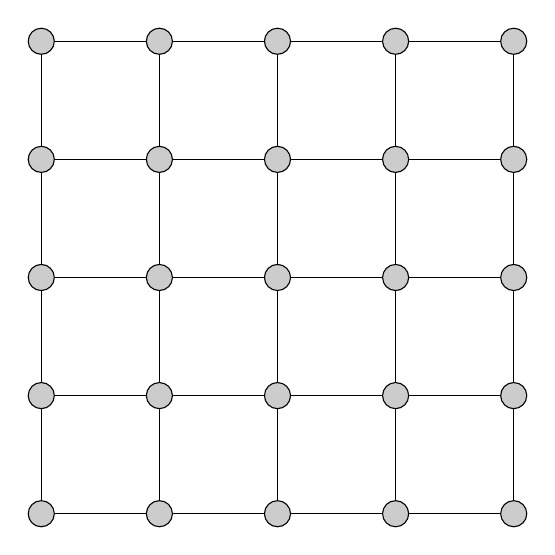
\begin{tikzpicture}[darkstyle/.style={circle,draw,fill=gray!40,minimum size=1}]
				\foreach \x in {0,...,4}
				\foreach \y in {0,...,4} 
				{\pgfmathtruncatemacro{\label}{\x - 5 *  \y +21}
					\node [darkstyle]  (\x\y) at (1.5*\x,1.5*\y) {};} 
				
				\foreach \x in {0,...,4}
				\foreach \y [count=\yi] in {0,...,3}  
				\draw (\x\y)--(\x\yi) (\y\x)--(\yi\x) ;
				
			\end{tikzpicture}
		\end{subfigure}
		\hfill
		\begin{subfigure}[b]{0.4\textwidth}
			\caption{Define distance: $D_{ab}=a(t) \Delta x_{ab}$, where \gls{gls:scale:factor} $a$ may or may not be a constant.}\label{fig:cosmo-1-distance}
			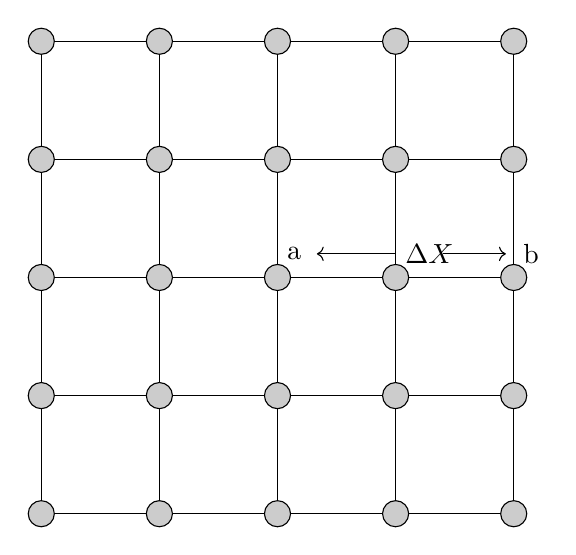
\begin{tikzpicture}[darkstyle/.style={circle,draw,fill=gray!40,minimum size=1}]
				\foreach \x in {0,...,4}
				\foreach \y in {0,...,4} 
				{\pgfmathtruncatemacro{\label}{\x - 5 *  \y +21}
					\node [darkstyle]  (\x\y) at (1.5*\x,1.5*\y) {};} 
				
				\filldraw[black] (1.5*2,1.5*2+0.3) node[anchor=west]{a}; 
				\filldraw[black] (1.5*4,1.5*2+0.3) node[anchor=west]{b}; 
				\filldraw[black] (1.5*3,1.5*2+0.3) node[anchor=west]{$\Delta X$}; 
				\draw[->]        (1.5*3+0.6,1.5*2+0.3)   -- (1.5*4-0.1,1.5*2+0.3);
				\draw[->]        (1.5*4-1.5,1.5*2+0.3)   -- (1.5*2+0.5,1.5*2+0.3);
				\foreach \x in {0,...,4}
				\foreach \y [count=\yi] in {0,...,3}  
				\draw (\x\y)--(\x\yi) (\y\x)--(\yi\x) ;
				
			\end{tikzpicture}
		\end{subfigure}
	\end{center}
\end{figure}
 
 We postulate a more general formula for distance between two galaxies $a$ and $b$:
 
 \begin{align*}            
 	D_{ab}=&a(t) \sqrt{\Delta_{ab} x^2 + \Delta_{ab} y^2 + \Delta_{ab} z^2}  \text{, where $a(t)$ is called the ''scale factor''}
\end{align*}
 Now calculate velocity:\footnote{\label{note1}During the lecture, $V$ is used for both velocity and volume. I will retain this usage in the notes; the reader should be careful to check which usage is meant.}           
 \begin{align*}	
 	V_{ab}=&\dot{a} \Delta X_{ab} \text{, neglecting $y$ and $z$}\\
 	\frac{V_{ab}}{D_{ab}} =& \frac{\dot{a}}{a} \text{, independent of choice of galaxies!}\\
 	=& H \text{, Hubble constant at a given time.}\\
 	V =& H D \text{, Hubble's Law.}
\end{align*}
 
\subsection{How much mass is in $\Delta x \Delta y \Delta z$?}

Assume  $\Delta x \Delta y \Delta z$ big enough that we can average over the small scale structure. How much mass is in there? Let $M$ denote the mass within $\Delta x \Delta y \Delta z$, and $M = \nu \Delta x \Delta y \Delta z$. Let $V$ denote the volume\textsuperscript{\ref{note1}}.

\begin{align*}
	V =& a^3 \Delta x \Delta y \Delta z\\
	M =& \nu \Delta x \Delta y \Delta z \text{, constant}\\
	\rho(t) =& \frac{\nu}{a(t)^3} \numberthis \label{eq:rho}
\end{align*}

Amount of mass in a given region of Figure \ref{fig:cosmo-1-grid} remains the same, as galaxies move with grid.

\subsection{Newtonian derivation of Friedmann's equation}
Choose grid so Newton is at rest at centre of universe. He looks out at distant galaxy, which moves in accordance with Newton's laws. He would use Newton's Theorem--Figure \ref{fig:newtons:thm} and Theorem \ref{thm:newton:shell}.

\begin{thm}[Newton's shell theorem]\label{thm:newton:shell}
	\begin{enumerate}
		\item A spherically symmetric body affects external objects gravitationally as though all of its mass were concentrated at a point at its center.
		\item If the body is a spherically symmetric shell (i.e., a hollow ball), no net gravitational force is exerted by the shell on any object inside, regardless of the object's location within the shell.
	\end{enumerate}
\end{thm}

\begin{proof}
	Given in \cite{enwiki:1241447151}.
\end{proof}

\begin{figure}[H]
	\caption[Newton's Theorem]{Newton's Theorem: to determine gravitational force on red body, assuming isotropy, draw sphere and calculate force as if mass inside shell were concentrated in centre, and ignore mass outside.}\label{fig:newtons:thm}
	\begin{center}
		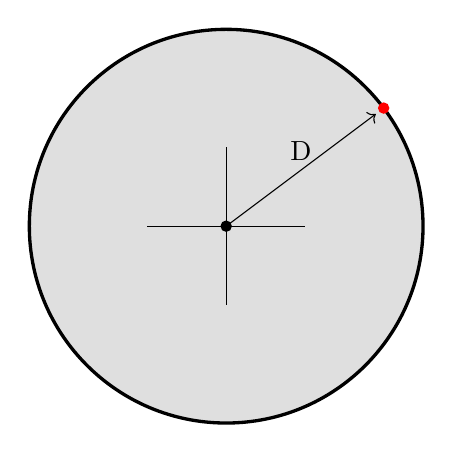
\begin{tikzpicture}[scale=0.5]
			\filldraw[color=black, fill=gray!25, very thick](0,0) circle (5.0);
			\filldraw[color=red, fill=red, very thick](4,3) circle (0.1);
			\filldraw[color=black, fill=black, very thick](0,0) circle (0.1);
			\draw[black] (-2,0) -- (2,0);
			\draw[black] (0,-2) -- (0,2);
			\draw[black,->] (0,0) -- (4*0.95,3*0.95) node[midway, above] {D};
		\end{tikzpicture}
	\end{center}
\end{figure}

\begin{align*}
	D =& a(t) \sqrt{x^2 + y^2 + z^2}\\
	=&a(t) R \text{, say} \numberthis \label{eq:D}
\end{align*}
R is constant, since galaxy is located at a fixed point in lattice. We want acceleration so we can use Newton's laws.
\begin{align*}
	V =& \dot{a(t)} R\\
	A =& \ddot{a(t)}R
\end{align*}
From Newton's Law of Universal Gravitation
\begin{align*}
	F =& - \frac{mMG}{D^2}\\
	A =& - \frac{MG}{D^2} \text{, which should become}\\
	=& \ddot{a(t)}R
\end{align*}
So we want
\begin{align*}
	\ddot{a(t)}R =& - \frac{MG}{D^2}\\
	=& - \frac{MG}{a^2 R^2} \text {, from \eqref{eq:D}}\\
	\frac{\ddot{a(t)}}{a} =& - \frac{MG}{a^3 R^3}\text{, now volume is}\\
	V =& \frac{4 \pi}{3}  a^3 R^3\\
	\frac{\ddot{a(t)}}{a}=& -\frac{4 \pi}{3} G \rho \text{, from definition of $\rho$} \numberthis \label{eq:a}
\end{align*}

Now $\rho$ does not depend in $R$, so \eqref{eq:a} applies for every galaxy. This is true for any origin, as long as we do the transformation carefully. Everything hinges on the assumption that the universe is homogeneous.

We can see from \eqref{eq:a} that the universe is not static unless $\rho=0$. Let us substitute \eqref{eq:rho} in \eqref{eq:a}.

\begin{align*}
	\frac{\ddot{a(t)}}{a} =& -\frac{4 \pi}{3} \frac{G \nu}{a^3}  \numberthis \label{eq:friedmann}
\end{align*}

This was discovered by Friedmann, in the context of General Relativity. It doesn't tell us whether universe is expanding or contracting, but tells us that acceleration is negative. But observation says that it isn't! This would have been the standard model before we found that expansion is accelerating.

\begin{figure}[H]
	\caption{Consider throwing rock up from Earth, along x-axis}\label{fig:cosmo:throw:rock}
	\begin{center}
		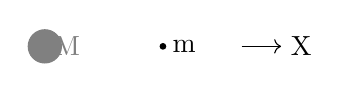
\begin{tikzpicture}[scale=0.5]
			\filldraw[gray] (0,0) circle (12pt) node[anchor=west]{M};
			\filldraw[black] (3,0) circle (2pt) node[anchor=west]{m};
			\draw [->] (5,0)   -- (6,0) node[right] {X};
		\end{tikzpicture}
	\end{center}
\end{figure}

We will write down the energy equation: total energy is $\frac{1}{2}m v^2 -\frac{m M G}{x}$. What is escape velocity if total energy is zero?
\begin{align*}
	\frac{1}{2}\cancel{m} V^2 -\frac{\cancel{m} M G}{X} =& 0\\
	V^2 =& \frac{2 M G}{X}
\end{align*}
Similarly in \eqref{eq:friedmann}, total energy can by positive, negative or zero.
\begin{itemize}
	\item If energy great enough, universe does not turn around: it expands forever.
	\item If energy smaller, universe eventually contracts.
	\item Escape velocity is the boundary between the other two cases.
\end{itemize}

In Figure \ref{fig:newtons:thm}, all the particle knows is that it is moving under influence of mass concentrated at origin, so we can treat as Figure \ref{fig:cosmo:throw:rock}.

The Total Energy is given by $\frac{1}{2} m \dot{a}^2 R^2 -\frac{m M G}{a R}$. In the edge case where energy is zero:
\begin{align*}
	 \dot{a}^2 R^2 -\frac{2 M G}{a R} =& 0 \\
	 \frac{\dot{a}^2 }{a^2} -\frac{2 M G \frac{4}{3} \pi}{\frac{4}{3} \pi a^3 R^3} =& 0 \\
	 {\underbrace{\big(\frac{\dot{a}}{a}\big)}_\text{Hubble}}^2 =& \frac{8 \pi}{3} G \rho \numberthis \label{eq:friedmann:eq}
\end{align*}
Equation \eqref{eq:friedmann:eq} is known as the Friedmann equation. This universe will get slower and slower, but never collapse.

Using \eqref{eq:rho}, \eqref{eq:friedmann:eq} becomes:
\begin{align*}
	\big(\frac{\dot{a}}{a}\big)^2 =& \frac{8 \pi \nu}{3}\frac{G}{a^3} \numberthis \label{eq:friedmann:8} \text{, or, using suitable units}\\
	\big(\frac{\dot{a}}{a}\big)^2 =& \frac{1}{a^3} \numberthis \label{eq:friedmann:8a}
\end{align*}
The right hand side of \eqref{eq:friedmann:8a} is always positive, and decreases as $a$ increases, but slows. We will attempt a trial solution, putting $a=ct^P$.
\begin{align*}
	a=&ct^P\\
	\dot{a}=&c P t^{P-1}\\
	\frac{\dot{a}}{a}=& \frac{P}{t} \text{. so \eqref{eq:friedmann:8a} becomes:}\\
	\frac{P^2}{t^2} =& \frac{1}{c^3 t^{3P}} \text{, whence}\\
	3P =& 2\\
	P =& \frac{2}{3}\\
	P^2 =& \frac{1}{C^3}
\end{align*}

\begin{figure}[H]
	\caption[Scale Factor]{Scale Factor, showing slowing (case discusses), collapsing, and real (accelerating) universes.}
	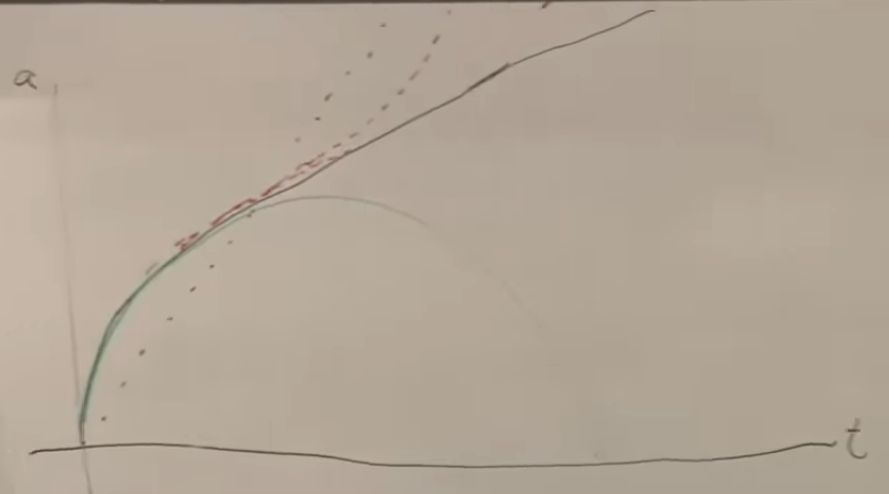
\includegraphics[width=\textwidth]{cosmo-1-scale-factor}
\end{figure}

Newton speculated about a homogeneous universe, but didn't carry out the calculation.

\section{Matter and radiation dominated universes} \label{sec:matter:radiation:dominated}

Did Newton get it right? Yes, mostly. Einstein's equations deal with curved space-time, and some of the universes we will study have curved 3-space, maybe a 3-sphere. Suppose we just look at very neighbouring galaxies, where it will look flat. Then in a small region we can use Newton;s equations. So what we did in Section \ref{sec:expanding:newton} should be OK, as long as we don't have two galaxies moving past each other at a speed comparable to that of light (But that is OK for galaxies that are a long way away).

Now photons and neutrinos are moving very fast, so  we have to modify our equations to deal with this.

Treat matter in galaxies as uniform density $\rho$. Lay down grid as in Figure \ref{fig:cosmo-1-grid}. How big is spacing? Equations should not depend on spacing, but maybe the ratios matter. If $a$ doubles, we have expansion.
\begin{figure}[H]
	\caption{Equations should not depend on spacing.}
	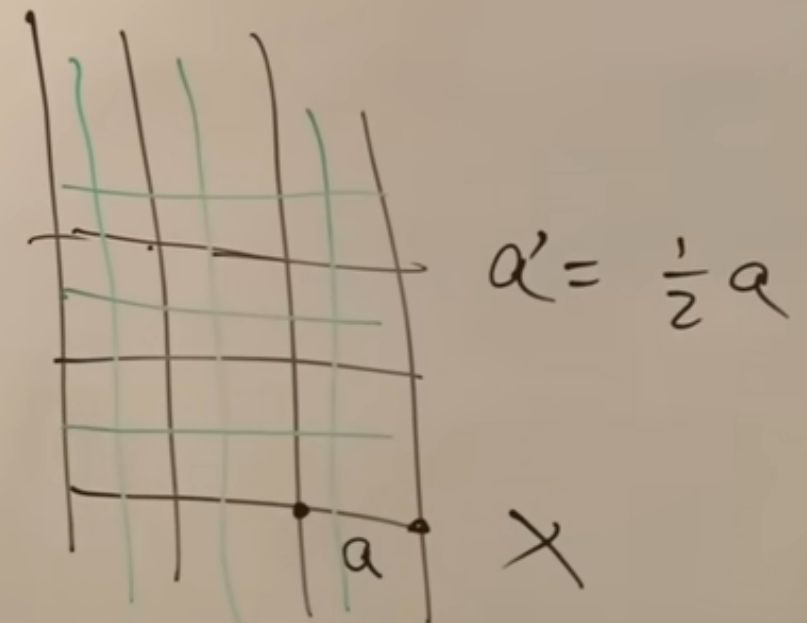
\includegraphics[width=0.8\textwidth]{cosmo-2-grid}
\end{figure}

We could measure expansion by $\frac{\dot{a}}{a}$.

Another ambiguity is $\nu$, which depends on $a$.

In Section \ref{sec:expanding:newton} we derived \eqref{eq:friedmann:8}, which reduces to:
\begin{align*}
	\big(\frac{\dot{a}}{a}\big)^2 =& \frac{8 \pi G \rho}{3}
\end{align*}

$\frac{8 \pi}{3}$ is related to the volume of a sphere. The equation assumes zero energy, or, equivalently, galaxies moving at escape velocity.

Is $\nu$ constant? If we assume, for the moment, that protons and galaxies are forever, then yes, $\nu$ is constant. Box grows, but number of particles in box remains constant. Recall \eqref{eq:friedmann:8}:
\begin{align*}
	\big(\frac{\dot{a}}{a}\big)^2 =& \frac{8 \pi \nu}{3}\frac{G}{a^3} \\
	\big(\frac{\dot{a}}{a}\big)^2 =& \frac{1}{a^3} \text{, using suitable units} \numberthis \label{eq:friedmann:normalized}
\end{align*}

We can solve \eqref{eq:friedmann:normalized}.

\begin{align*}
	\dot{a} =& \frac{1}{\sqrt{a}}\\
	\frac{dt}{da} =& \sqrt{a} \text{, $\pm$ corresponds to expansion/contraction} \\
	t = \frac{2}{3}a^{\frac{3}{2}}\\
	a = t^\frac{2}{3} \text{, ignoring some constant} \numberthis \label{eq:2:3}
\end{align*}

\begin{figure}
	\caption[Decelerating growth of scale parameter]{Scale parameter increases with time, but decelerates as the result of gravitational attraction}
	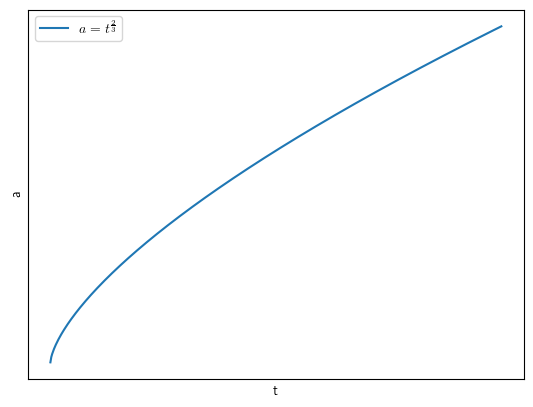
\includegraphics[width=0.8\textwidth]{cosmo-2-a-t}
\end{figure}


	
NB. Real motion of galaxies is made up of flow plus \gls{gls:peculiar:velocity}.

There are two directions we want to go in.
\begin{enumerate}
	\item What if we replace matter with photons? (Early universe). Section \ref{sec:radiation:dominated}
	\item What if energy is non-zero?--Section \ref{sec:matter:dominated}.
\end{enumerate}

\subsection{Matter dominated universe}\label{sec:matter:dominated}
\begin{figure}[H]
	\caption{We compute the constant energy}
		\begin{center}
			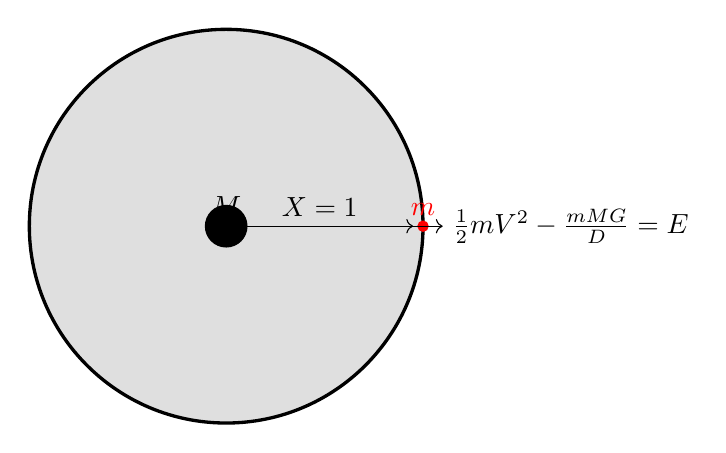
\begin{tikzpicture}[scale=0.5]
				\filldraw[color=black, fill=gray!25, very thick](0,0) circle (5.0);
				\filldraw[color=red, fill=red, very thick](5,0) circle (0.1) node[right,above]{$m$};
				\filldraw[color=black, fill=black, very thick](0,0) circle (0.5) node[above]{$M$};
				\draw[black,->] (0,0) -- (5*0.95,0) node[midway, above] {$X=1$};
				\draw[black,->] (5*0.95,0) -- (5.5,0) node[right] {$\frac{1}{2}m V^2 - \frac{mMG}{D}=E$};
			\end{tikzpicture}
	\end{center}
\end{figure}

\begin{align*}
	 V^2 -  \frac{2MG}{D} =& \frac{2E}{m}\\
	 D =& aX \\
	 V =& \dot{a} X \text{, but we have set $X=1$}\\
	 D =& a \\
	 V =& \dot{a} \text{, so the energy equation becomes}\\
	 \dot{a}^2 - \frac{2MG}{a} =& C \text{, say}\\
	 \big(\frac{\dot{a}}{a}\big)^2 - \frac{2MG}{a^3} =& \frac{C}{a^2} \\
	 \big(\frac{\dot{a}}{a}\big)^2 - \frac{8\pi\rho G}{3} =& \frac{C}{a^2}\\
	 \big(\frac{\dot{a}}{a}\big)^2  =& \frac{8\pi\nu G}{3a^3} + \frac{C}{a^2} \text{, on substituting \eqref{eq:rho}} \numberthis \label{eq:full:friedmann}
\end{align*}

Equation \eqref{eq:full:friedmann} is the full Friedmann equation, which he derived from General Relativity; we have derived from Newton.

if $C>0$, right hand side is strictly positive, universe continues to grow forever (For if $\dot{a}>0$ initially, it has to pass through zero to stop expanding). If $a$ small enough $\frac{8\pi\nu G}{3 a^3}$ will dominate, and we can use \eqref{eq:2:3}. Once $a$ grows enough $ \frac{C}{a^2}$ dominates.

\begin{align*}
	\big(\frac{\dot{a}}{a}\big)^2  =&  \frac{C}{a^2} \\
	\frac{\dot{a}}{a} =&  \frac{C}{a} \text{, for some new $C$}\\
	\dot{a} =& C
\end{align*}

Eventually we can neglect gravity and velocity is uniform.

What if energy is negative? Equation \eqref{eq:full:friedmann} becomes:

\begin{align*}
	\big(\frac{\dot{a}}{a}\big)^2  =& \frac{8\pi\nu G}{a^3} - \frac{C}{a^2} \text{, for some new, positive $C$}
\end{align*}
Now there is a point where $\dot{a}=0$: the expansion stops, and $\dot{a}$ changes from positive branch of square root to negative.

\begin{figure}[H]
	\caption{Negative Energy:  there is a point where $\dot{a}=0$}
	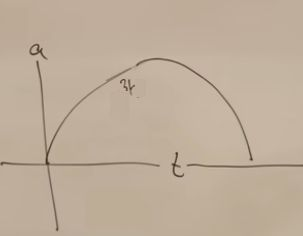
\includegraphics[width=0.8\textwidth]{cosmo-2-negative}
\end{figure}

The matter dominated universe was the classic cosmology until other things were discovered. There are three cases, positive energy, negative and zero. In a later lecture we will find that this is connected to the geometry of the universe: this is the main contribution of General Relativity.


\subsection{Radiation dominated universe}\label{sec:radiation:dominated}

We do have to think about relativity, but there is only one important thing: $E=mc^2$. We rewrite Equation \eqref{eq:full:friedmann} to show the connection with general relativity, and define $\gls{gls:kappa} = C$:

\begin{align*}
	\underbrace{\big(\frac{\dot{a}}{a}\big)^2  - \frac{\gls{gls:kappa}}{a^2}}_\text{Terms involving geometry}=& \underbrace{\frac{8\pi}{3} G \rho}_\text{Matter and energy} \numberthis \label{eq:geometry:energy}
\end{align*}
We'll replace mass density with energy density. Energy = $Mc^2 + $ Radiation (and we will choose units such that $c=1$).

To compute radiation density, take a box, volume $a^3$, and assume a certain number of photons.

\begin{figure}[H]
	\caption{Unit box with photons: \gls{gls:lambda} increases as box expands adiabatically }\label{fig:unit:box}
	\begin{center}
			\begin{subfigure}[t]{0.45\textwidth}
				\begin{center}
					\caption{As box expands adiabatically, photons do work on walls of box. Number of photons does not change.}
					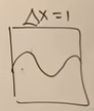
\includegraphics[width=\textwidth]{cosmo-2-unit-box}
				\end{center}
			\end{subfigure}
			\;
			\begin{subfigure}[t]{0.45\textwidth}
				\begin{center}
					\caption{An analogy with standing waves. Number of nodes (zero crossings) is an adiabatic invariant:  it has to be an integer. So $\gls{gls:Lambda}$ stretches with circle.}
					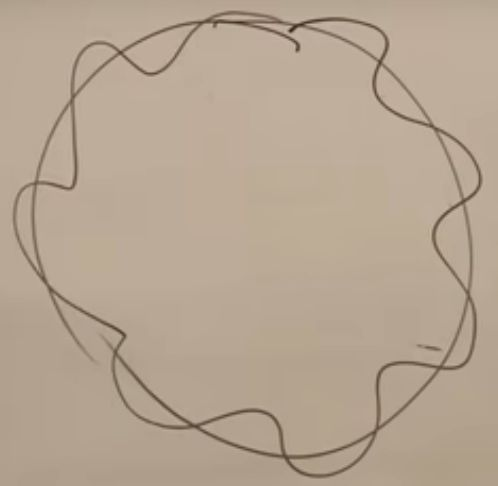
\includegraphics[width=\textwidth]{cosmo-2-standing-waves}
				\end{center}
			\end{subfigure}	
	\end{center}
\end{figure}

\begin{align*}
	V =& a^3\\
	E =& \frac{h c}{\gls{gls:Lambda}}
\end{align*}

We have to do some more quantum mechanics of classical electromagnetism to justify the statement in Figure \ref{fig:unit:box}. For the time being, take it as a given. So energy in box decreases: $E\propto \frac{1}{a}$ and $\rho\propto \frac{1}{a^4}$. We substitute in \eqref{eq:geometry:energy}:

\begin{align*}
	\big(\frac{\dot{a}}{a}\big)  =& \frac{8\pi\nu G}{a^4} - \frac{C}{a^2} \text{, and explore the case where $C=0$}\\
	\big(\frac{\dot{a}}{a}\big)  =& \frac{8\pi\nu G}{a^4} \text{, or, with suitable units}\\
	\big(\frac{\dot{a}}{a}\big)  =& \frac{1}{a^4} \text{, taking square root and rearranging} \\
	\dot{a} =& \frac{1}{a}\\
	\frac{dt}{da} =& a\\
	t =& a^2 \text{, in suitable units}\\
	a =& \sqrt{t} \numberthis \label{eq:a:scrt:t}
\end{align*}

\begin{figure}[H]
	\caption[Comparison of radiation and matter dominated universes]{Comparison of radiation and matter dominated universes--\eqref{eq:2:3} and \eqref{eq:a:scrt:t}}\label{fig:cosmo-2-a-r}
	\begin{center}
			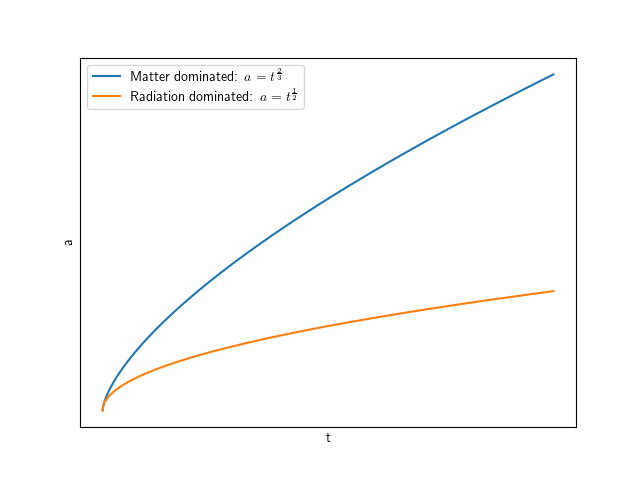
\includegraphics[width=0.8\textwidth]{cosmo-2-a-r}
	\end{center}
\end{figure}


\subsection{Mixed case: neither matter nor radiation dominates}

We consider a real universe with both matter and radiation.

\begin{align*}
	\big(\frac{\dot{a}}{a}\big)^2 =& \underbrace{\frac{C_m}{a^3}}_\text{More important for big $a$} + \underbrace{\frac{C_R}{a^4}}_\text{More important for small $a$}
\end{align*}

At start of expansion, radiation dominates, $t^{\frac{1}{2}}$, but later switches, $t^{\frac{2}{3}}$--Figure \ref{fig:cosmo-2-a-r}.

\begin{itemize}
	\item How do we know that there isn't conversion of matter to energy as universe expands? In practice mostly conserved separately once things cool to 1000K.

	\item There is a third component: dark energy (dark matter is included in $C_m$).

	\item Radiation includes photons, gravitons, and neutrinos, which move at speeds close to $c$.
\end{itemize}

This is the cosmology of 30 years prior to date of lecture (2013).

What happens to radiation energy lost during expansion?
\begin{align*}
	\underbrace{- \big(\frac{\dot{a}}{a}\big)^2}_\text{Kinetic Energy} + \frac{C_m}{a^3} +\frac{C_R}{a^4} =& 0 
\end{align*}

Kinetic Energy is  tiny at present.

There are two ways to think about time translation symmetry.
\begin{enumerate}
	\item The universe is a time dependent thing that everything moves in. There is no longer time translation symmetry, so energy doesn't have to be conserved.
	\item There is time translation symmetry: starting universe at $t=-7$ is exactly that same as starting at $t=4$, but this adds an extra term to energy equation. This is very subtle and we'll discuss later.
\end{enumerate}

There are three cases in \eqref{eq:geometry:energy}.

\begin{align*}
	\big(\frac{\dot{a}}{a}\big)^2  =& \frac{8\pi\rho G}{3} - \frac{\gls{gls:kappa}}{a^2} 
\end{align*}

In Section \ref{sec:geometries}, we will see that $\gls{gls:kappa}$ is connected with geometry.
\begin{itemize}
	\item If $\gls{gls:kappa}=0$, space is flat.
	\item If $\gls{gls:kappa}>0$, space is curved like a sphere, and it compact.
	\item If $\gls{gls:kappa}<0$, space is curved negatively.
\end{itemize}


\section{Geometries of space: flat, spherical, hyperbolic} \label{sec:geometries}

As a matter of observation, space \emph{is} flat. We don't know that it is flat, just that it is very big, and we don't know whether there is any curvature. It is important to investigate the various possibilities. We don't know what is happening on scales beyond 10 billion light years, but we will make some assumptions. We won't assume that it is flat, but we will assume that it is homogeneous and isotropic. Is that true? We don't know, but we can only test it if we know its consequences. Almost all cosmology is based on that assumption.

If space is not flat, it must be curved. While there are many types of curved spaces, most are not compatible with the universe being \gls{gls:homogenous}.

\begin{itemize}
	\item A parabaloid is most certainly not homogeneous. Its curvature is greater at the tip, less further away.
	\item A long pointy ellipsoid is not homogeneous. You would notice the difference if you were walking around on it.
	\item Surfaces with bumps are not homogeneous.
\end{itemize}

What kinds of spaces \emph{can} be curved and homogeneous? There are two kinds, positive curvature, Section \ref{sec:positive:curvature}, and negative, Section \ref{sec:negative:curvature}.

\subsection{Flat Space and the 3-sphere}\label{sec:positive:curvature}

Let's think about a metric for ordinary flat space, restricting to 2 dimensions.

\begin{align*}
	ds^2 =& dx^2 + dy^2\text{, or changing to polar coordinates}\\
	=&dr^2 + r^2 d\theta^2 \text{, or changing notation}\\
	=&dr^2 + r^2 d\Omega_1^2 \numberthis \label{eq:flat:polar}
\end{align*}

Use the idea that $d\theta^2$ is a  metric for $\Omega_1$, the 1-sphere or unit circle.

\begin{figure}[H]
	\caption[We can treat a circle as a piece of string and deform it]{We can treat circle as a piece of string and deform it. Label by angular coordinate so equal distances map to the equal angles. A circle is just a curve where we come back to the same place after an angle of $2\pi$.}
	\begin{center}
		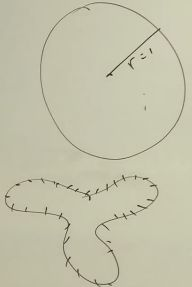
\includegraphics[width=0.8\textwidth]{cosmo-3-1-sphere}\label{fig:cosmo-3-1-sphere}
	\end{center}
\end{figure}

In polar coordinates, it \emph{looks} as if there is a special place, but, in reality, all points are the same. We will think of flat 2d space as a nested collection of circles--\eqref{eq:flat:polar}. 

The 2-sphere is also homogeneous. Every point on the surface of the sphere is the same as any other point. It has uniform curvature. If you walk around you come back to the same space.

\begin{figure}[H]
	\caption[Nested spheres with point indicating observer]{Nested spheres with point indicating observer. Observer looks out and sees a series of nested spheres, maybe one light year apart. They start growing, slow down, and then contract. Characterize spheres by angle $r$. We will denote the 2-sphere $\Omega_2$.} 
	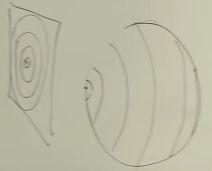
\includegraphics[width=0.8\textwidth]{cosmo-3-1-nested-spheres}
\end{figure}

The metric of the 2-sphere is:

\begin{align*}
	d\Omega_2^2 =& dr^2 + \sin^2 r\; d\Omega_1^2
\end{align*}

This pattern just continues. If I want to make a 3 dimensional sphere--a 3 dimensional space where every point is the same, and where we eventually come back to the same point. If we look into space for a certain distance, things form a 2-sphere. Look further, a bigger 2-sphere, but eventually they start to get smaller.

\begin{figure}[H]
	\caption[Nested 2-spheres in a 3-sphere]{Nested 2-spheres in a 3-sphere. The observer is in the 3-sphere, at the point $r=0$. The 2-spheres surround the observer.}
	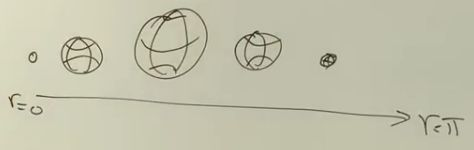
\includegraphics[width=0.8\textwidth]{cosmo-3-3-sphere}
\end{figure}

The metric follows the familiar pattern:
\begin{align*}
	d\Omega_3^2 =& dr^2 + \sin^2 r\; d\Omega_2^2
\end{align*}

What happens in flat space? In polar coordinates, \eqref{eq:flat:polar} generalizes to:
\begin{align*}
	ds^2 =& dr^2 + r^2 d\Omega_2^2
\end{align*}

There is another way to view spheres. Imagine an ant living on a circle. It can receive light along the circle, it can communicate with its neighbours, but it has no way of knowing whether it lives on either curve in Figure \ref{fig:cosmo-3-1-sphere}, or even whether there are additional dimensions. We, however, can describe a circle by embedding it in two dimensions.
\begin{figure}[H]
	\caption{Embedding an $n$-sphere in $n+1$ dimensions}
	\begin{subfigure}[t]{0.5\textwidth}
		\caption{A 1-sphere in two dimensions}
		\begin{tikzpicture}
			\draw[fill=none](0,0) circle (2.0) node [above,right] {};
			\node[] at (1.8,1.9) {$x^2 + y^2 = 1$};
			\draw[->](-2.5,0) -- (2.5,0) node [above] {$x$};
			\draw[->](0,-2.5) -- (0,2.5) node [above] {$y$};
		\end{tikzpicture}
	\end{subfigure}
	\begin{subfigure}[t]{0.5\textwidth}
		\caption{A 2-sphere in three dimensions}
		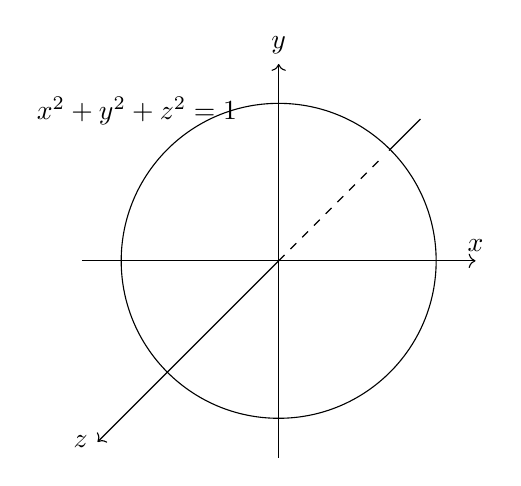
\begin{tikzpicture}
			\draw[fill=none](0,0) circle (2.0) node [black] {};
			\node [] at (-1.8,1.9) { $x^2 + y^2 + z^2= 1$};
			\draw[->](-2.5,0) -- (2.5,0) node [above] {$x$};
			\draw[->](0,-2.5) -- (0,2.5) node [above] {$y$};
			\draw[->](0,0) -- (-2.3,-2.3) node [below,left] {$z$};
			\draw[dashed](0,0) -- (1.3,1.3) node [below,left] {};
			\draw[](1.4,1.4) -- (1.8,1.8) node [below,left] {};
		\end{tikzpicture}
	\end{subfigure}
\end{figure}
Similarly we can embed a 3-sphere in 4 dimensions: $x^2 + y^2 + z^2+w^2= 1$. We don't have to answer the question whether this makes physical sense.


What is the difference in what we perceive between a sphere and an infinite flat plane? Suppose we had telescopes that allow us to determine the distance to distant objects. The telescope doesn't measure $r$, but there are tricks, e.g. spectroscopy, brightness(assume galaxies the same). We ask what angle they subtend. 

\begin{figure}[H]
	\caption{Standard Galaxies in flat space}
	\begin{subfigure}[t]{0.45\textwidth}
		\caption{Standard galaxy has width $d$}
		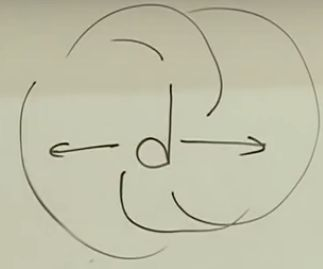
\includegraphics[width=\textwidth]{cosmo-3-3-standard-galaxy}
	\end{subfigure}
	\begin{subfigure}[t]{0.45\textwidth}
		\caption{For flat space, the observer perceives the width of the galaxy to be $ds^2 = r^2$, so $d\theta^2 = d^2$}
		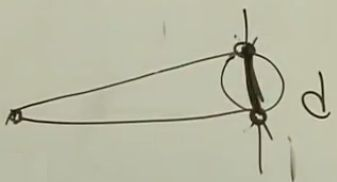
\includegraphics[width=\textwidth]{cosmo-3-3-standard-galaxy-flat-space}
	\end{subfigure}
\end{figure}

Now, consider the 2-sphere.

\begin{figure}[H]
	\caption{Galaxies embedded in 2-sphere, with observer at "left pole".}
	\begin{center}
		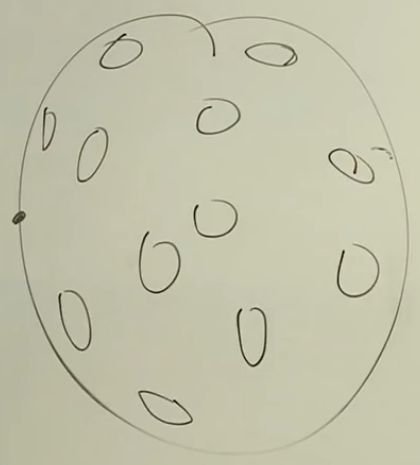
\includegraphics[width=0.6\textwidth]{cosmo-3-galaxies-2-sphere}
	\end{center}
\end{figure}

\begin{align*}
	d^2 =& \sin^2 r d\theta^2\\
	d\theta =& \frac{d}{\sin r}
\end{align*}

$d\theta$ is bigger than if we lived in flat space. Distant galaxies appear bigger, but fainter. So we can distinguish flat and spherical.

We can also count the number of galaxies: on  a sphere you see fewer galaxies at great distances, compared to the plane. At antipodes we see just one galaxy.

\begin{figure}[H]
	\caption[Stereographic Projection]{Stereographic Projection: observer is at South pole. Every point on sphere projects to a point on plane, and North pole projects to infinity. Circles on sphere map to little closed curves on plane (actually circles).}
	\begin{center}
			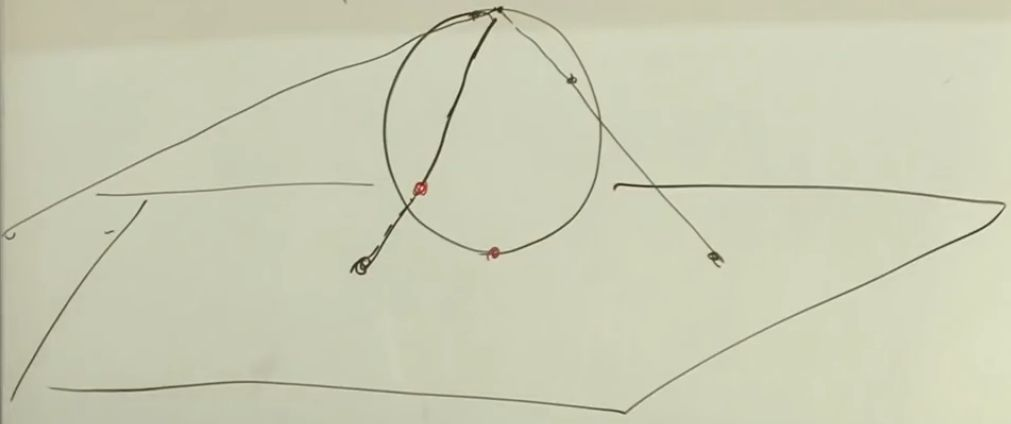
\includegraphics[width=0.6\textwidth]{cosmo-3-stereographic-projection}
	\end{center}
\end{figure}

How do circles on the plane map to circles on the sphere? If they are close to South pole they look the same. As we move further the projections get bigger, and the extreme Arctic circle looks very large. Sphere is homogeneous, but this doesn't match plane. 

We can do the same thing with a 3-sphere.

\subsection{Hyperbolic geometry}\label{sec:negative:curvature}
There is a third homogeneous geometry, which we'll call the hyperbolic space. As we move from observer, size of circles blows up very rapidly.

\begin{align*}
	d\mathcal{H}_2^2 =& dr^2 + \sinh^2 r d\Omega_1^2\\
	d\mathcal{H}_3^2 =& dr^2 + \sinh^2 r d\Omega_2^2 \text{, candidate geometry for our space.}
\end{align*}

What happens to angle subtended by a galaxy?

\begin{align*}
	d\theta	 =& \frac{d}{\sinh r}\\
	\approx& \frac{2d}{e^r}
\end{align*}
So if we lived in a hyperbolic universe, we'd notice that distant galaxies looked to small, and there were a lot of them.

We will construct the hyperbolic surface $T^2-x^2-y^2=1$.

\begin{figure}[H]
	\caption{Hyperboloid. }
	\begin{subfigure}[t]{0.3\textwidth}
		\caption{This doesn't appear \emph{homogeneous}, but is if we use metric $t^2-x^2-y^2$ (Lorentz Transformation)}
		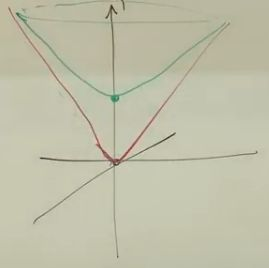
\includegraphics[width=\textwidth]{cosmo-3-hyperboloid}
	\end{subfigure}
	\;
	\begin{subfigure}[t]{0.3\textwidth}
		\caption{Stereographic projection. We project points onto plane. Notice asymptotic circle: there are no points outside this. There is a lot of distortion.}
		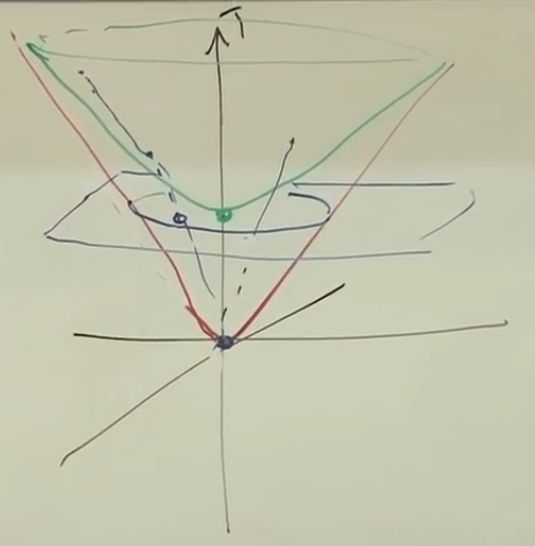
\includegraphics[width=\textwidth]{cosmo-3-hyperboloid-stereographic}
	\end{subfigure}
	\;
	\begin{subfigure}[t]{0.3\textwidth}
		\caption{The angels and devils are supposed to be the same size, and each one sees the same things, and has the same neighbours. There are coordinate transformation that will map one onto the other.}
		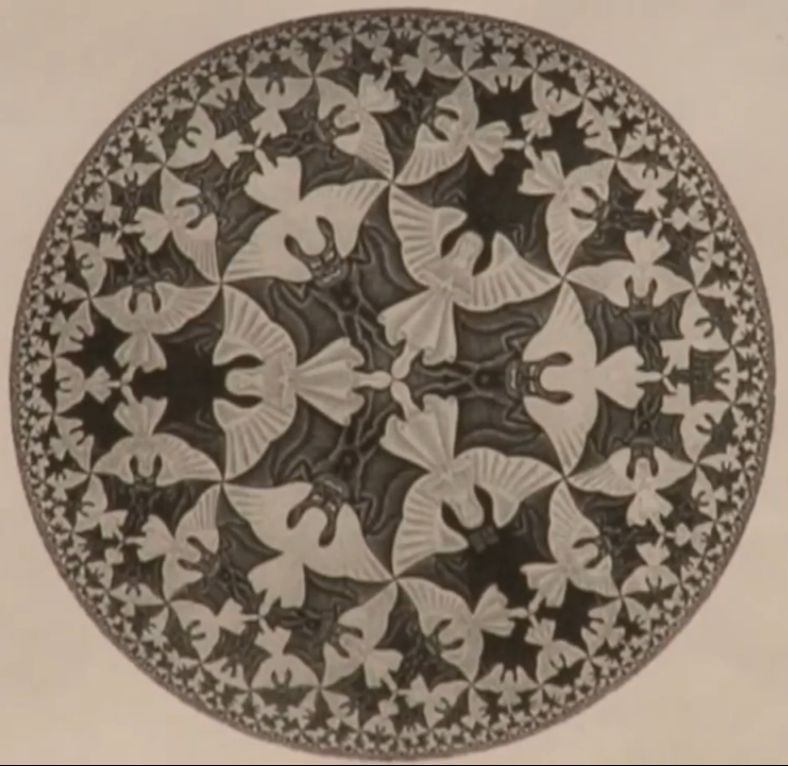
\includegraphics[width=\textwidth]{cosmo3-escher}
	\end{subfigure}
\end{figure}

This geometry has many names. It is also the uniformly negatively curved space.

We can also make the space have a radius other than 1.
\begin{align*}
	ds^2 =& a^2 \big(dr^2 + \sin^2 r d\Omega_{n-1})^2\big) \text{sphere} \\
	ds^2 =& a^2 \big(dr^2 + \sinh^2 r d\Omega_{n-1})^2\big) \text{hyperboloid}
\end{align*}
The smaller $a$, the greater the curvature.

Modern cosmology assumes that the space we live in is one of the three that we have considered.  On scales that we can currently detect, the Universe appears flat--out to 22 billion light years, so we know that the radius must be at least 10 times this side.

Space could also be a torus, a rectangle with opposite sides identified; flat, with periodic boundary conditions. People have looked for evidence of periodicity, but not found any\footnote{This was in response to a question asked at the start of Section \ref{sec:cosmological:thermodynamics}}.
 
 \subsection{Space and Time}\label{sec:space:time}
 
 The Minkowski metric is:
 \begin{align*}
 	ds^2 = - dt^2 + dx^2 + dy^2 + dz^2 
 \end{align*}
 
 A light ray (null ray) is $ds^2$=0--$dx=\pm dt$
 
 We will replace $ dx^2 + dy^2 + dz^2 $ with one of the metrics we have discussed, e.g.
  \begin{align*}
 	ds^2 =& - dt^2 + a(t)^2d\Omega_2^2\\
 	D =& a(t) \theta\\
 	V =& \dot{a}\theta\\ 
 	=& \frac{\dot{a}}{a} D \text{, Hubble Law}
 \end{align*}
 
  Space is 2 dimensional, and diameter of space changes with time, $2+1$
  
 Here are our 3 cases of interest:
 \begin{align*}
 	ds^2 =& -dt^2 + a(t)^2 \big( dx^2 + dy^2 + dz^2 \big) \text{, Flat, but scale factor depends on time}\\
 	ds^2 =& - dt^2 + a(t)^2d\Omega_3^2 \text{, spherical, with varying radius}\\
 	ds^2 =& - dt^2 + a(t)^2d\mathcal{H}_3^2 \text{, hyperbolic, with varying radius}
 \end{align*}

We need to investigate how $a$ varies with time. We will need to write down equations from General Relativity. It turn out they will agree with the Friedmann equations we derived from Newtonian physics.
\section{Cosmological Thermodynamics}\label{sec:cosmological:thermodynamics}


\subsection{Questions from audience}
\subsubsection{if universe is expanding, how come planets maintain stable orbits?}

Hold hands out in space with friend. There is a very mild repulsion from expansion, but repulsion is dwarfed by holding hands. Also atoms closer together, so attraction dominates Hubble attraction. Consider at atom, which is also embedded in space. Electrostatic forces overwhelm expansion. Atom will be expanded a tiny bit, but not enough to fly apart. Same is true of the solar system: gravitational pull of Sun overwhelms tendency to expand.

Energy conservation in an expanding universe is different from energy conservation in a static universe. The simplest way to look at is is to note that energy conservation is a consequence of time translation invariance: if everything is time invariant, we get energy conservation. If background is not static, energy conservation does not apply. Nett amount of energy isn't fixed: changes in energy translate into kinetic energy of expansion.

NB: Homogeneity and isotropy is on a large scale; things are not homogeneous out to a few hundred million light years.

\subsubsection{Clarification of homogeneity}

Homogeneity means that it is possible to write the metric so that it has the same form anywhere. Consider  2 dimensional flat space:
\begin{align*}
	ds^2 =& dx_1^2 + dx_2^2 \text{. Suppose we translate the coordinates}\\
	\vec{y} =& \vec{x} + \vec{a} \text{. Then in the new coordinates}\\
	ds^2 =&dy_1^2 + dy_2^2 \text{, which has the same form.}
\end{align*}

We can show that a similar thing happens with $ds^2=dr^2 + \sin^2 r d\theta^2$ if we move observer from South pole to East pole. In 2 dimensions it is enough that the curvature be the same at every point. The hyperbolic surface is also homogeneous and isotropic. The torus is also translation invariant, but not isotropi.c, because of there being preferred directions.

Being homogeneous and isotropic is somewhere between being a postulate and an observational fact.

Geometry has its own intrinsic shape, it isn't necessarily embedded. In 1 dimension the only thing that matters is distance along the curve. And they are not curved: we straighten any piece. They are flat but closed.

What is special about 3 dimensions? Our brain architecture evolved to navigate a 3 dimensional space. Mathematically 3 dimensional space isn't special.

\subsection{Setting up the Geometry}


Let us assume that space has one of the 3 homogeneous and isotropic geometries described in Section \ref{sec:space:time}.

General Relativity starts with a metric, and we will assume that space and time aren't mixed with each other in the metric\footnote{This is a consequence of homogeneity and isotropy}. The metric has one of these three forms:
\begin{align*}
	ds^2 =& - dt^2 + a(t)^2 d\Omega_3^2 &\gls{gls:kappa}=1\text{, or}\\
	ds^2 =& - dt^2 + a(t)^2 \big(dx^2 + dy^2 +dz^2\big) &\gls{gls:kappa}=0\text{, or}\\
	ds^2 =& - dt^2 + a(t)^2 d\mathcal{H}_3^2 &\gls{gls:kappa}=-1	\text{ }
\end{align*}
In all three cases:
\begin{align*}
	D =& a(t) d\theta\\
	V =&  \dot{a} d\theta\\
	=& \frac{\dot{a}}{a}D	
\end{align*}

Hubble's parameter $\frac{\dot{a}}{a}$ depends on time, but not on position.

\subsection{Einstein's Field Equation}

From \cite[Lecture 9]{susskind2012general}:
\begin{align*}
	\underbrace{R^{\mu\nu} - \frac{1}{2}g^{\mu\nu}R}_\text{Einstein Tensor}=&\underbrace{\frac{8\pi G}{3}}_\text{c.f. equation \eqref{eq:full:friedmann}}\underbrace{ T^{\mu\nu}}_\text{Energy-momentum} \numberthis \label{eq:einstein:field}
\end{align*}

$T^{\mu\nu}$ contains a complex of things: the density of energy. the flux of energy, the density of momentum, and the flux of momentum. We will fix on the time-time component\footnote{This turns out to give Newton's energy equation; other components would give $F=mA$.}, $\frac{8\pi G}{3} T^{00}$. $T^{00}$ is the energy density, $\rho$, so we will write $\frac{8\pi G}{3} \rho$. The right hand side is completely sensitive to the type of material that is in the universe, e.g. matter, photons: it knows about the material that makes up the universe.

The curvature has two parts, one of which involves second derivatives of the metric by the coordinates, the other squares of first derivatives. Fortunately the time-time component contains only one of the two: the second derivatives cancel, and we only have squares of first derivatives.

There are derivatives by time, and by space. The space ones are connected with curvature of space, which scales as $\frac{1}{R}$; the time ones with how things are changing with time, i.e. $a(t)$. Einstein's Field Equation, \eqref{eq:einstein:field}, reduces to:

\begin{align*}
	\big(\frac{\dot{a}}{a}\big)^2 + \frac{\gls{gls:kappa}}{a^2}=& \frac{8\pi}{3} \rho \text{, or}\\
	\big(\frac{\dot{a}}{a}\big)^2 =& \frac{8\pi G}{3}\rho - \frac{\gls{gls:kappa}}{a^2} \text{, c.f. Equation \eqref{eq:geometry:energy}} \numberthis \label{eq:einstein:equation}
\end{align*}

We can interpret $\gls{gls:kappa}$ as curvature, rather than energy.

Why does General Relativity give the same answer as Newton? If we just look at a small region of curved space, it looks flat. Once we realize that equations are the same for a small piece and a large one, we see that we must reproduce Newton's equations. In Newton's view, $\rho$ is the mass density, which if accurate if everything is moving at speeds much less than light. On the other hand, the Einstein equations are more general than Newton's: they apply to fast moving particles, and photons.

\subsection{Equation of State}\label{sec:equation:state}

We need to understand how $\rho$ depends on $a$ to solve \eqref{eq:einstein:equation}. We will consider two cases:
\begin{align*}
	\rho=&\frac{\rho_0}{a^3} \text{, Matter dominated, and} \numberthis \label{eq:matter:eos}\\
	\rho=&\frac{\rho_0}{a^4} \text{,  Radiation dominated} \numberthis \label{eq:radiation:eos}
\end{align*}

There are also combinations of these two.

We will proceed in two steps:
\begin{enumerate}
	\item Assume an equation of state, and use it to derive equations like \eqref{eq:matter:eos} and \eqref{eq:radiation:eos}.
	\item Derive equation of state for different kinds of materials.
\end{enumerate}

An equation of state is a relationship between thermodynamic variables describing a system. For our system, temperature won't play a big role. We will be interested in the relationship between energy density and pressure. The example of interest can be described by very simple equations of state.

\begin{align*}
	P =& w \rho\text{, for some constant $w$} \numberthis \label{eq:p:w:rho}\\
	w =& 0 \text {, for a matter dominated universe}\\
	w =& \frac{1}{3} \text{, radiation dominated--see \eqref{eq:w:1:3}}
\end{align*}

Consider a box of gas. We can work out the total energy from the density and volume, $V$.
\begin{align*}
	E =& \rho V \numberthis \label{eq:E:rho:V}
\end{align*}
 
We change the volume, doing work. From \cite{susskind2013statistical}[Lecture 6], assuming an adiabatic change:

\begin{align*}
	dE =& -P dV + \underbrace{T dS}_\text{$=0$} \numberthis \label{dE:PdV:TdS}\\
	=& \rho dV + V d\rho \text{, from \eqref{eq:E:rho:V}. Combine with \eqref{dE:PdV:TdS}}\\
	V d\rho =& -\big(p+\rho\big)dV \numberthis \label{eq:Vdrho}
\end{align*}
(It is permissible to add $p$ and $\rho$ as the latter is \emph{energy} density. Both have dimension $\mathsf{T^{-2}L^{-1}M}$.)
\begin{align*}
	V d\rho =& - (1+w)\rho dV \text{, from \eqref{eq:p:w:rho} and \eqref{eq:Vdrho}. Regrouping}\\
	\frac{d\rho}{\rho} =& - (1+w)\frac{dV}{V} \text{, and integrating}\\
	\rho =& \frac{C}{V^{1+w}}\\
	=& \frac{C}{a^{3(1+w)}}\numberthis \label{eq:rho:a}
\end{align*}

\begin{itemize}
	\item If $w=0$, we have a matter dominated universe, with $\rho=\frac{C}{a^3}$
	\item If $w=\frac{1}{3}$, we have a radiation  dominated universe, with $\rho=\frac{C}{a^4}$
\end{itemize}

We need little more than the equation of state to derive a universe.

\subsection{Dark Energy, Cosmological Constant, Vacuum Energy}

Let's try $w=-1$. (E.g Replace box with a line interval with a spring joining the ends. Pressure is negative\footnote{We call this tension}, as spring is drawing ends together. Increasing potential energy makes pressure more negative.) Then $\rho$ is constant: it does not change when box expands.

We can mock up the cosmological constant by adding linear term to Newton's gravitational law.

\section{Vacuum energy}

What is the history of the Universe? To the extent that it homogeneous and isotropic, this question boils down to the time history of the scale factor. If we know the history of the scale factor we know an awful lot about the history of the universe. We can test it, and observe it.

We have looked at \begin{itemize}
	\item the matter dominated universe, in  which $a(t)\propto t^{\frac{2}{3}}$--Equations \eqref{eq:2:3}\&\eqref{eq:matter:eos}, 
	\item energy dominated $a(t)\propto t^\frac{1}{2}$--Equations \eqref{eq:a:scrt:t} \& \eqref{eq:radiation:eos}.
\end{itemize}

Both are models, and neither is absolutely correct. We believe that the second model was approximately correct for the early universe, and that the first became true later. We will discuss when we get to observational cosmology.

We also looked at the relation between $a$ and $\rho$--Equation \eqref{eq:rho:a}. \begin{itemize}
	\item $\rho =\frac{\rho_0}{a^3}$ (matter dominated),
	\item  $\rho =\frac{\rho_0}{a^4}$, radiation dominated.
\end{itemize}

The equation of state is $P = w\rho$--Equation \eqref{eq:p:w:rho}. In a matter dominated universe, because $E=mc^2$, a tiny amount of mass still has a large energy density. But particles have a low velocity; where does pressure come from? From particles hitting the wall, slowly; so formula for pressure contains velocities of particles, but not $c$. It is much less than energy density, so $w=0$ for a non-relativistic matter dominated universe. For radiation, $w=\frac{1}{3}$, which we will prove in Section \ref{sec:w:1:3}.

\subsection{Why is $w=\frac{1}{3}$?}\label{sec:w:1:3}

Radiation is massless particles--photons. Figure \ref{fig:cosmo-5-box-photons} depicts a box of photons.

\begin{figure}[H]
	\caption{A box of photons}
	\begin{subfigure}[t]{0.55\textwidth}
		\caption{Photons bounce of walls, lose no energy, and exert pressure on walls}\label{fig:cosmo-5-box-photons}
		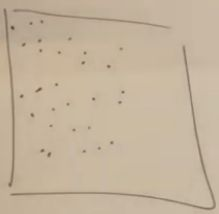
\includegraphics[width=\textwidth]{cosmo-5-box-photons}
	\end{subfigure}
	\begin{subfigure}[t]{0.4\textwidth}
		\caption{Photon hitting wall at angle $\theta$}\label{fig:cosmo-5-wall}
		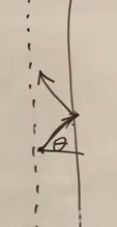
\includegraphics[width=\textwidth]{cosmo-5-wall}
	\end{subfigure}
\end{figure}


Let us pretend that all photons have the same energy (we will find out this doesn't matter; it is approximately true of photons are in thermal equilibrium). Let:
\begin{itemize}
	\item energy per photon be $\epsilon$;
	\item  momentum per photon $\vec{\pi}$, (not "the" $\pi$), and 
	\item number of photons per unit volume be $\nu$.
\end{itemize}

In any little volume of box, on average momentum could be in any direction (isotropic).
\begin{align*}
	\epsilon =&  \pi c \text{, where }\\
	\pi=&\lvert\vec{\pi}\rvert \text{, so}\\
	\epsilon =& \pi \text{, in units where $c=1$}
\end{align*}
Let number of photons per unit volume be $\nu$. Then the energy density is:
\begin{align*}
	\rho =& \nu \epsilon 
\end{align*}

How many particles hit the box during time interval $\Delta t$? In Figure \ref{fig:cosmo-5-wall}, a particle moving to right will hit the wall during $\Delta t$ if it is close enough--within $\Delta X$--where $\Delta X=\Delta T$. What if it is not moving exactly right, say at angle $\theta$--Figure \ref{fig:cosmo-5-wall}?
\begin{align*}
	\Delta x =& \Delta t \, \cos{\theta} \text{. Then the momentum will change by:}\\
	\Delta_{\pi} =& 2 \epsilon \cos {\theta} \text{, since particle turned around, so}\\
	\frac{\Delta_{\pi}}{\Delta t} =& \frac{2 \epsilon \cos {\theta}}{\Delta t} \text{, is the force per particle that hits wall}
\end{align*}
Now the number of particles that hit the wall is given by
\begin{align*}
	N =& \frac{1}{2}\Delta x A \nu \text{, where $A$ is area, and $c=1$}
\end{align*}
allowing for the fact that half the particles within $\Delta x$ are moving away. We now calculate the contribution to the pressure from particles moving at angle $\theta$
.\begin{align*}
	P(\theta) =& \frac{1}{2} \frac{2 \epsilon \cos {\theta}}{\Delta t} \Delta x  \; \nu \text{, force per area}\\
	=& \frac{\cancel{2}}{\cancel{2}}  \epsilon \cos {\theta} \Delta x  \nu \text{, force per area}\\
	=&  \epsilon \nu \cos^2 {\theta}  \\ 
	=& \rho  \cos^2 {\theta} 
\end{align*}
Now integrate over all $\theta$. We shall suppose that every direction is characterized by a unit vector $\vec{n}$, Figure \ref{fig:cosmo-5-nxnynz}.

\begin{figure}[H]
	\caption{Unit vector $\hat{n}$}\label{fig:cosmo-5-nxnynz}
	\begin{center}
		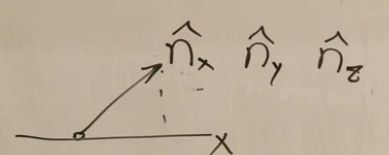
\includegraphics[width=0.6\textwidth]{cosmo-5-nxnynz}
	\end{center}
\end{figure}

We see that:
\begin{align*}
	n_x =& \cos{\theta}\\
	\hat{n}_x^2 +  \hat{n}_y^2 +  \hat{n}_z^2=&1
\end{align*}
Now $n_x$, $n_y$, and $n_z$ are related by rotational symmetry. We can take average over 3D space, and use isotropy to get:
\begin{align*}
		\langle \hat{n}_x\rangle^2 + \langle \hat{n}_y\rangle^2 + \langle \hat{n}_z\rangle^2=&1\\
	P =&\frac{1}{3} \rho \text{, or}\\
	w =& \frac{1}{3}\text{, as asserted in Section \ref{sec:equation:state}}\numberthis \label{eq:w:1:3}
\end{align*}

We assumed all particles have the same energy. If not, we could interpret \eqref{eq:w:1:3} as the contribution from a particular energy, and integrate over all energies.

What wall are we talking about? There is no wall in space. Really they are going right through, but, on average there is one coming from the opposite direction, so, on average, our argument works for thermal equilibrium (\gls{gls:cmb} is in thermal equilibrium).

\subsection{Vacuum Energy}
Can energy density ever be negative? Yes, but not under any circumstances we will be interested in. (Yes it can). Pressure can be negative--tension: two ends connected by a spring. If pressure negative and $\rho$ positive, we have negative $w$. (LS would not bother unless it were central to cosmology.) If particles are attractive they can give negative pressure.

Vacuum energy comes from quantum field theory, and gives rise to negative pressure. It is an energy that we assign to empty space (zero point energy of fluctuation). A box contains a vacuum energy equal to vacuum energy density times volume.

The vacuum energy density is a constant; it is independent of $a(t)$:
\begin{align*}
	\rho_0 =& \gls{gls:Lambda} \frac{3}{8 \pi G}
\end{align*}

$\gls{gls:Lambda}$ is known as the ''cosmological constant'', or as ''dark energy''. For the significance of the factor $\frac{3}{8 \pi G}$, see \eqref{eq:full:friedmann}

We shall work out the equation of state.
\begin{align*}
	E =& \rho_0V\\
	dE =& \rho_0 dV \\
	=&-w \rho_0 dV \text{ from \eqref{eq:p:w:rho}, whence}\\
	w=&-1
\end{align*}

When you read that astronomers are measuring $w$, and discovering that $w$ is close to $-1$, they are talking about vacuum energy. The closer the experimental evidence is to $w=-1$, they are saying that the energy of the universe is like vacuum energy; it doesn't dilute, because it is a property of empty space.

Vacuum energy can be positive or negative, but, in both cases, pressure and density have opposite sign. We don't know the value of $\rho_0$: there are too many contributions.

Let us study the case where the vacuum energy density is the \emph{only} density. Earlier we look at a pure matter dominated universe, Section \ref{sec:matter:dominated}, and now we'll look at a pure vacuum energy universe. There are six cases for non-zero $\gls{gls:Lambda}$ and  for $\gls{gls:kappa}$--Table \ref{table eq:options:lambda:kappa}.

The Friedmann equation, \eqref{eq:full:friedmann}, becomes:
\begin{align*}
	\big(\frac{\dot{a}}{a}\big)^2  =& \frac{8\pi G}{3} \rho_0 - \frac{\gls{gls:kappa}}{a^2}\\
	=& \gls{gls:Lambda} - \frac{\gls{gls:kappa}}{a^2} \numberthis \label{eq:friedmann:avec:lambda}
\end{align*}

\begin{table}[H]
	\begin{center}
		\caption{Options for $\gls{gls:Lambda}$ and \gls{gls:kappa}}\label{table eq:options:lambda:kappa}
		\begin{tabular}{||l|l|p{5cm}||} \hline
			$\gls{gls:Lambda}$ & $\gls{gls:kappa}$ & Remarks\\ \hline
			0 & +1 & Already done\\\hline
			0 & 0 & Already done\\\hline
			0 & -1 & Already done\\\hline
			+1 & 0 &de Sitter space--see Section \ref{sec:lambda:pos:k:0}\\\hline
			+1 & +1 &de Sitter space--see Section \ref{sec:lambda:pos:k:1} \\\hline
			-1 & +1 & Makes no sense as it would make $\big(\frac{\dot{a}}{a}\big)^2<0$\\\hline
			-1&-1&Section \ref{sec:neg:neg} \\\hline
			\hline
		\end{tabular}
	\end{center}
\end{table}

\subsubsection{Flat space, positive cosmological constant}\label{sec:lambda:pos:k:0}

Substituting  $\gls{gls:Lambda}>0$ and $\gls{gls:kappa}=0$ in Friedmann's equation \eqref{eq:friedmann:avec:lambda} gives:
\begin{align*}
	\big(\frac{\dot{a}}{a}\big)^2  =& \gls{gls:Lambda}\\ 
	\dot{a} =& \sqrt{\gls{gls:Lambda}} a\\
	a(t) \propto& e^{\sqrt{\gls{gls:Lambda}}t} \text{, universe expands exponentially}
\end{align*}
 The Hubble constant is $\sqrt{\gls{gls:Lambda}}$, and $
 a(t) \propto e^{Ht}$. This is known as ''de Sitter space''.
 
 Let us mix in some matter:
 \begin{align*}
 	\big(\frac{\dot{a}}{a}\big)^2  =& \gls{gls:Lambda} + \frac{C}{a^3}
 \end{align*}
 
 In early times, $a$ is small, and $\frac{C}{a^3}$ will dominate; later, $a$ is large and $\gls{gls:Lambda}$ will dominate. Right now the two energies compete (for last 2-3 billions years, dark energy has started to become more important. Observation shows that it is accelerating, and, as precision increases, it looks more like exponential acceleration. )
 
 Positive vacuum energy comes from bosons, negative from fermions. LS says it is a mystery that vacuum energy is so low.
 
 \subsubsection{Positive curved space, positive cosmological constant}\label{sec:lambda:pos:k:1}
 
 Substituting $\gls{gls:Lambda}>0$ \& $\gls{gls:kappa}>0$ in the Friedmann equation, \eqref{eq:full:friedmann}, gives:
 \begin{align*}
 	\big(\frac{\dot{a}}{a}\big)^2  =& \gls{gls:Lambda} - \frac{1}{a^2}\\
 	\dot{a}^2 - \gls{gls:Lambda} a^2 =&-1
 \end{align*}
 Think of $a(t)$ as the coordinate of a particle on a line. $\dot{a}^2$ becomes twice the kinetic energy; $-\gls{gls:Lambda} a^2$ the potential energy plotted in Figure \ref{fig:cosmo-5-pe}. Think of $a$ starting large, going up hill, then rolling back. 
 
 
 We can solve to get:
 \begin{align*}
 	a(t) =& \frac{1}{\sqrt{\gls{gls:Lambda}}} \cosh {(\sqrt{\gls{gls:Lambda}}t)}
 \end{align*}
 
 \begin{figure}[H]
 	\caption{$\dot{a}^2 - \gls{gls:Lambda} a^2 =-1$}
 	 \begin{subfigure}[t]{0.45\textwidth}
 		\caption{Potential Energy}\label{fig:cosmo-5-pe}
 		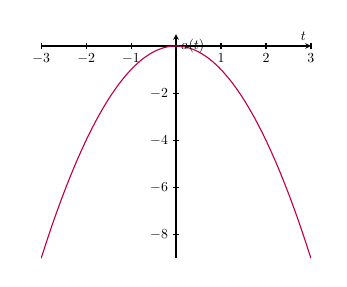
\begin{tikzpicture}[scale=0.5]
 			\begin{axis}[
 				trig format=rad, % HERE
 				xlabel = $t$,
 				ylabel = $a(t)$,
 				xmin = -3,xmax = 3,
 				ymin = -9,ymax = 0.5,
 				domain = -3:3,
 				smooth,thick,
 				axis lines = middle,
 				every tick/.style = {thick}]	
 				\addplot[color=purple]{-x*x};		
 			\end{axis}
 		\end{tikzpicture}
 	\end{subfigure}
 	\;
 	\begin{subfigure}[t]{0.45\textwidth}
 		\caption{'$a(t) = \frac{1}{\sqrt{\gls{gls:Lambda}}} \cosh {(\sqrt{\gls{gls:Lambda}}t)}$'}
 		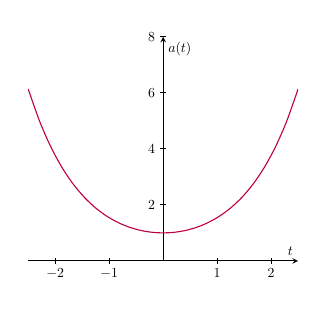
\begin{tikzpicture}[scale=0.5]
 			\begin{axis}[
 				trig format=rad, % HERE
 				xlabel = $t$,
 				ylabel = $a(t)$,
 				xmin = -2.5,xmax = 2.5,
 				ymin = 0,ymax = 8,
 				domain = -2.5:2.5,
 				smooth,thick,
 				axis lines = middle,
 				every tick/.style = {thick}]	
 				\addplot[color=purple]{cosh(x)};		
 			\end{axis}
 		\end{tikzpicture}
 	\end{subfigure}
 \end{figure}
 
\begin{figure}[H]
	\caption{Universe bounces at $t=0$}
	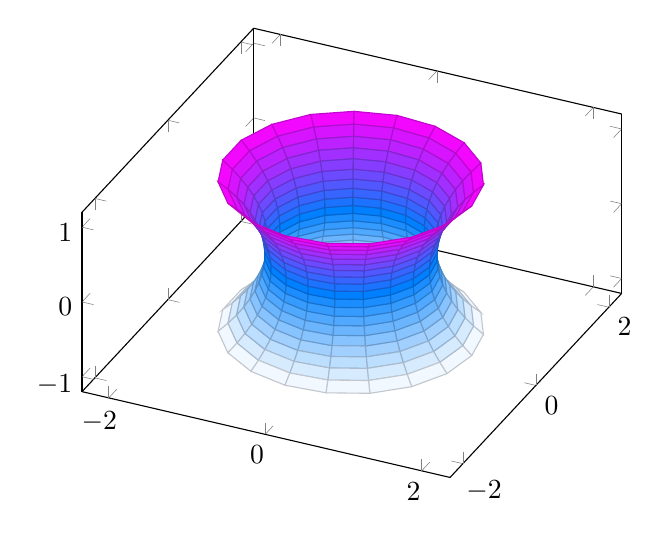
\begin{tikzpicture}	
		\begin{axis}[axis equal]
			\addplot3 [surf,
			colormap/cool, %colour scheme
			domain=0:360, %sets range for x
			y domain=-1:1, %sets range for y
			samples=20, %number of samples taken
			z buffer=sort]
			(
			{cos(x)*cosh(y)},
			{sin(x)*cosh(y)},
			{y}
			);
		\end{axis}
	\end{tikzpicture}
\end{figure}
 
 \subsubsection{Negative cosmological constant, with negative curvature}\label{sec:neg:neg}
 We will consider a negative cosmological constant, with negative curvature:
 
 The Friedmann equation, \eqref{eq:full:friedmann}, becomes:
 \begin{align*}
 	\big(\frac{\dot{a}}{a}\big)^2  =& -1 + \frac{1}{a^2} \\
 	\dot{a}^2 + a^2 =&1 \text{, the energy equation for a harmonic oscillator}
 \end{align*}
 
 Universe expands and crunches.
 


\section{Dark matter and allocation of energy density}

We will look at the connection between experimental facts and our models.

\subsection{Review}
\begin{align*}
	\big(\frac{\dot{a}}{a}\big)^2 =& H^2 \text{, Friedmann, Hubble}\\
	=& \frac{8\pi G}{3} \rho - \frac{\gls{gls:kappa}}{a^2}
\end{align*}

This changes with time: when people speak of the ''Hubble constant'' they mean today's value.

Our metric is:
\begin{align*}
	ds^2 =& - dt^2 +a(t)^2\big[dr^2 + \xi^2(r) d\Omega^2\big] \text{, where} \numberthis \label{fig:metric:6}\\
	\xi(r)=&\sin{r}& \text{ if } \gls{gls:kappa} = +1\\
	\xi(r)=&\sinh{r}& \text{ if }\gls{gls:kappa} = -1\\
	\xi(r)=&r& \text{ if } \gls{gls:kappa} = 0
\end{align*} $\xi$ depends on the geometry.

There are only 3 contributions to $\rho$ known.

\begin{align*}
	- \frac{\gls{gls:kappa}}{a^2} + \frac{8 \pi G}{3}\rho = \underbrace{\frac{C_R}{a^4}}_\text{Radiation} + \underbrace{\frac{C_M}{a^3}}_\text{Matter}+ \underbrace{\gls{gls:Lambda}}_\text{Vacuum energy} - \frac{\gls{gls:kappa}}{a^2}\\
	=&H^2 \numberthis \label{eq:hubble:contraint}
\end{align*}

Equation \eqref{eq:hubble:contraint} is a constraint. Each term has some value, as does $H$. How do we measure them?

\begin{itemize}
	\item Hubble determined his constant by plotting red-shift against luminosity. He miss-measured by a factor of 10. We do better today, and we look at a small enough part of universe that we don't have to worry about age varying.

	\item What about $C_R$? We can look at the amount of radiation in universe, mostly in \gls{gls:cmb}, but it isn't very big.

	\item Matter, we look at the galaxies, and see how much hydrogen is in them, measure luminosity, and measure luminous matter. It comes to one proton per cubic metre. Low, but much higher than radiation density.
	
	\item Forget vacuum energy for the time being. We are being historical, so leave out dark matter and dark energy.
\end{itemize}

Today we call the ratios $\Omega_R$, $\Omega_m$, $\Omega_{\gls{gls:Lambda}}$, and $\Omega_{\gls{gls:kappa}}$,normalized so:
\begin{align*}
	\Omega_R+\Omega_m+\Omega_{\gls{gls:Lambda}}+\Omega_{\gls{gls:kappa}}=&1
\end{align*}

When LS was a student, $\Omega_R$ was negligible, $\Omega_{\gls{gls:Lambda}}$ was unknown, and Hubble constant was 20 times larger than $\Omega_m$, so it was assumed that $\Omega_{\gls{gls:kappa}}\approx 1$. The meant on open, infinite universe with $k\approx -1$. For most of the time $\frac{c_M}{a^3}$ competes favorably with $\frac{\gls{gls:kappa}}{a^2}$

$H$ has another meaning in a matter dominated universe, where $a\propto t^\frac{2}{3}$. Also:
\begin{align*}
	\frac{\dot{a}}{a}=&\frac{2}{3t}\\
	H=&\frac{2}{3t}\\
	H_{today}=&\frac{2}{3T}\\
	\approx& 10^{10} \text{ years}
\end{align*}

We also have (From where?)
\begin{align*}
	\frac{1}{a^2} =& \frac{1}{H^2} \text{, so} \\
	a \propto& T
\end{align*}
 None of this is true: it is what they thought 40 years ago.
 
\subsection{Dark Matter}
Ordinary matter is made from luminous matter: it radiates when it gets hot. In 1932 Oort noticed some galaxies were misbehaving, and, the following year, Zwicky noticed some clusters of galaxies were misbehaving: things were not moving the way Newton's laws predicted, unless there was a great deal of mass that was not accounted for. Black holes aren't massive enough; moreover, Oort realized that the extra mass could not be concentrated at the centre.

Most of the luminous matter is in the centre of the galaxy, so the outer parts should move under a central force.

\begin{figure}[H]
	\caption[Most of the luminous matter is in the centre of the galaxy]{Most of the luminous matter is in the centre of the galaxy, so the outer parts should move under a central force.}
	\begin{subfigure}[t]{0.45\textwidth}
		\caption{A star moving under a central force}
		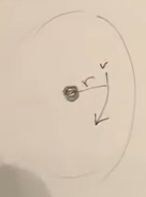
\includegraphics[width=\textwidth]{cosmo-6-galaxy}
	\end{subfigure}
	\begin{subfigure}[t]{0.45\textwidth}
		\caption{Observed velocity is constant, unlike predicted velocity}\label{fig:cosmo-6-velocity-curve}
		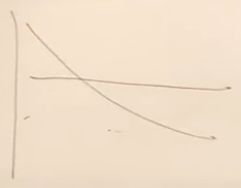
\includegraphics[width=\textwidth]{cosmo-6-velocity-curve}
	\end{subfigure}	
\end{figure}

\begin{align*}
	\frac{MG}{r^2} =& \frac{v^2}{r}\\
	v^2 \propto \frac{1}{r} \text{, Kepler}
\end{align*}
But this isn't what is observed--Figure \ref{fig:cosmo-6-velocity-curve}: velocity (not angular velocity) is pretty much constant. Newton would have assumed mass is distributed in 3D in accordance with some function $M(r)$

\begin{align*}
	\frac{M(r)G}{r^2} =& \frac{v^2}{r}\\
	\frac{M(r)G}{r} =& v^2 \text{, but $v$ is constant, so}\\
	M(r) \propto& r
\end{align*} 

\subsubsection{Dark Matter}
So $M$, not $\rho$, increases linearly, at least out to the boundary of the galaxy. LS does not know of a good argument why mass behaves this way. Observation of stars to top and bottom of galaxy suggests that distribution is spherical, and it is ten times mass of luminous mass.

Why doesn't it collapse? Luminous matter lost energy by radiation. Dark matter isn't changed, and particles are very light.

LS suggest that dark matter clumped first, then baryons were clumped also and lost energy through radiation. Black holes didn't play [much of a] part.

Why not neutrinos? They are so light they'd need to move very fast (''hot dog matter''), but dark matter tends to cluster.

Dark matter didn't make the discrepancy with the Hubble constant go away, but it lessened it.

Dark matter can't be fermions  if they are light, but maybe bosons. Bose condensate? (garbled!)

\subsubsection{Modify gravitational theory}

The alternative is to modify gravitational theory Newton's laws to that  Kepler's 2nd law doesn't work for galaxies, but this doesn't seem to work.
Most physicists think it is particles. Since Newtonian gravity works find in our solar system, we know that ordinary matter dominates here. Matter in solar system is much denser than interstellar space.

\subsection{Testing cosmological theories}

How do we test the following equation?

\begin{align*}
	\frac{C_M}{a^3} - \frac{\gls{gls:kappa}}{a^3} = H^2
\end{align*}

A model consists of $\gls{gls:kappa}$ and an equadrtion of state, for which we can substitute a history, $a(t)$. We can measure red-shift, and luminosity.

To start, assume we can ignore time. how can we measure $\gls{gls:kappa}$? Meausure number of galaxies of a given brightness, as a function of distance.

\begin{itemize}
	\item In a flat space, the number of galaxies in a shell of thickness $dr$ goes as $r^2$.
	\item In a hyperbolic space, the number of galaxies in a shell of thickness $dr$ goes as $\sinh^2(r)$, which is exponential, $e^{2r}dr$
	\item In a 3-sphere, the number of galaxies in a shell of thickness $dr$ goes as $\sin^2(r)$
\end{itemize}

The evidence favours a hyperbolic space, as a function of red-shift. What about luminosity?
\begin{itemize}
	\item In flat space, luminosity falls of as $\frac{1}{r^2}$
	\item In hyperbolic space, luminosity falls mush faster.
\end{itemize}

What about number of galaxies as a function of red-shift?

Let $\gls{gls:Lambda}_{e}mitted$ denote the wavelength of light is emitted from a source. This may or may not be the wavelength that is detected: Doppler shift is one possible reason; gravitational shift due to a black hole is another; expansion of the universe is equivalent to the Doppler shift, but it is what we are interested in.

\begin{figure}[H]
	\caption[Map of the Universe]{Map of the Universe. Vertical lines correspond to equal values of $r$, wavy line is light ray, and we see a number of galaxies. They have different  scale factors, $a(t)$: c.f. $a_{TODAY}$. Light emitted at point with $a(t)$ has to stretch to get to where we observe it, by a factor of $\frac{a_{TODAY}}{a_t}$.}
	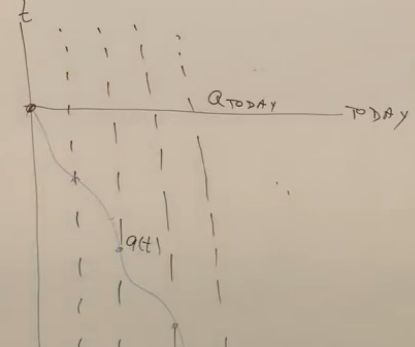
\includegraphics[width=0.8\textwidth]{cosmo-6-map-universe}  
\end{figure} 

\begin{defn}[Redshift]
	\begin{align*}
		z =& \frac{\gls{gls:Lambda}_{Detected}}{\gls{gls:Lambda}_{Emitted}}-1 \text{, $-1$ for historical reasons}\\ 
		=&\frac{a_{TODAY}}{a_t} - 1 \numberthis \label{eq:z:a}
	\end{align*}
\end{defn}


Each galaxy we observe at a different distance was emitted at a different time, and has its own redshift. But until we know how the light ray moves, we don't know how to compare scale factors.

A light ray is a null ray for the metric \eqref{fig:metric:6}. If a light ray is moving radially towards us, $dt^2=a(t)^2dr^2$. This has two solutions, one going back into the past (the one we are interested in), and one going to the future. The past solution is:

\begin{align*}
	dt=&-a(t)dr\text{, as $t$ gets more negative, $r$ get bigger} \\
	dr=&-\frac{dt}{a(t)}\numberthis \label{eq:dr:dt}
\end{align*}

Let us invent something an astronomer can test: what is $\frac{dN}{dz}$, the number of galaxies per unit redshift.

\begin{align*}
	\frac{dN}{dz} \propto& \frac{dr \xi(r)^2}{dz}\\
	dz =& -\frac{a_{TODAY}}{a(t)^2}da\\
	\frac{dN}{dz} \propto& \frac{dr  \xi(r)^2}{-\frac{a_{TODAY}}{a(t)^2}\dot{a}dt}\\
	\propto& \frac{ \xi(r)^2}{-\frac{a_{TODAY}}{a(t)^2}\dot{a}}\frac{dr}{dt}\\
	\propto& \frac{\xi(r)^2}{\frac{a_{TODAY}}{a(t)}\dot{a}} \text{, from \eqref{eq:dr:dt}}\\
	\propto&\frac{\xi(r)^2}{(z+1)\dot{a}} \text{, from \eqref{eq:z:a}} \numberthis \label{dN:dz}
\end{align*}

There is nothing we can do with this until we make a model. We will take the matter dominated universe, and set $\gls{gls:kappa}=-1$.

\begin{align*}
	a \propto& t^\frac{2}{3}\\
	\dot{a}& \frac{2}{3}t^\frac{1}{3}
\end{align*}

Now $a$, $\dot{a}$, $r$ can all be expressed in terms of $z$, so we can express the right hand side of \eqref{eq:z:a} in terms of $z$ (only because we have a model). Now $\xi(r)$ increases exponentially, which is easy to detect: it makes an anomalously large galaxies\footnote{Galaxies is used to mean standard candles, and the best ones are supernovae} at large redshift. You can convert a $\gls{gls:kappa}$ and equation of state\footnote{The $\Omega s$ form part of the model.} into a prediction for the number of galaxies at a given redshift. Given this, and the relationship between luminosity and redshift we can work out the complete history of the universe, and determine $C_R$.

 Observations over the last 50 years are inconsistent with matter dominated universe with negative $\gls{gls:kappa}$. Best fit today is:
 \begin{align*}
 	\Omega_R=&0\\
 	\Omega_m\approx&0.3 \text{ including dark matter}\\
 	\Omega_{\gls{gls:Lambda}}\approx&0.7\\
 	\Omega_{\gls{gls:kappa}}\approx&\pm0.01\\
 \end{align*}
If you vary these numbers by more than one percent, model fails to match data. Also we can determine $\Omega_R$ and $\Omega_m$ (subject to assumption about dark matter), so we only need to search on other two.

The values above are today's values:
\begin{itemize}
	\item Long in the past $\Omega_R\approx1$; 
	\item long in the future $\Omega_{\gls{gls:Lambda}}\approx1$
\end{itemize} 


We get a $\pm 10\%$ model with supernova data; add in the \gls{gls:cmb} we get $\pm 1\%$.

\section{Temperature History of the Universe}

\subsection{Review}
Last week we saw that the best way to estimate the rough parameters of the expanding universe is to begin with a model, then calculate its consequences; if that doesn't work so well, adjust parameters and keep going until we agree with data. The model consists of a time history for the scale factor, and a specification for the geometry. Until we get to the \gls{gls:cmb} and its details, we typically don't see deep enough and far enough that the $\gls{gls:kappa}$ is critical to our analysis. Counting galaxies and supernovae with redshifts that are no bigger than 7, they aren't sensitive to curvature. That is both good and bad: it is bad because we can't deduce the curvature; but since it isn't sensitive to curvature, we don't need to know its value to work out the history of the scale factor. We can work out the relationship between brightness and distance, and the number of objects with a given redshift. Data is consistent with negligible curvature and about 70\% dark energy.

We have to look deep into \glsdesc{gls:cmb} to get more.

\subsection{Black Body Radiation}

Temperature is a feature of thermal equilibrium. Thermal equilibrium is a condition for a system that is established after a period of time by scattering.

Let's imagine a box with perfectly reflecting walls and put photons into it. Open wee hole, shine laser in, then close hole. If photons don't interact, box won't come into thermal equilibrium. We need \emph{scattering} to get thermal equilibrium. Charged particles will scatter effectively. If box has some electrons, photons will scatter, electrons will scatter, and particles will eventually form a thermal soup; we could say that the box has a temperature.

The universe appears to be electrically neutral: $\gls{gls:n:electrons}=\gls{gls:n:proton}$. Hydrogen atoms aren't effective scatterers, so today the universe is not in thermal equilibrium, or the different kinds of particles aren't in thermal equilibrium with each other. If electrons and protons weren't bound, they would be efficient scatterers, and the universe would have a well defined temperature. We need a high temperature to ensure they aren't bound.

Returning to our box, we have a temperature $T$, and each photon has an wavelength \gls{gls:lambda} and frequency \gls{gls:nu} (there are many different wavelengths in the box).

Radiation is characterized by the intensity: $I(t,\nu)dVd\nu$ is energy per unit volume in band of frequencies $d\gls{gls:nu}$. First attempt (before 1900), using dimensional analysis.
\begin{align*}
	dim \; I(t,\nu) =& \big[\frac{E T}{V}\big]
\end{align*}

What are units of temperature--i.e. energy per particle? $E = \gls{gls:kB}T$ (Boltzmann's constant is just a conversion factor: temperature can be treated as energy). We can ask what sort of dependence $I$ can have on $T$ and \gls{gls:nu}? The only thing that will work dimensionally is:


\begin{align*}
	I \propto & \frac{T \gls{gls:kB} \nu^2}{c^2} \numberthis \label{eq:raleigh:jeans}
\end{align*}

This a a disaster: $I$ grows without bound as \gls{gls:nu} grows, and the energy in the box is infinite. We need another constant to avoid the ''ultraviolet catastrophe''. The correct formula for black body radiation is:
 
\begin{align*}
	I =& \frac{2 h \nu^3}{c^2} \frac{1}{e^\frac{h\nu}{\gls{gls:kB}T}-1} \numberthis \label{eq:planck:black:body}
\end{align*}

For small \gls{gls:nu}, \eqref{eq:planck:black:body} reduces to \eqref{eq:raleigh:jeans}, and for  $\frac{h\nu}{\gls{gls:kB}T} \gg 1$ it behaves more like $e^\frac{-h\nu}{\gls{gls:kB}T}$, averting the ultraviolet catastrophe.

At the crossover point
\begin{align*}
	\frac{h\nu}{\gls{gls:kB}T} =& 1 \text{, or}\\
	\frac{hc}{\gls{gls:kB}T} =& \gls{gls:lambda} \text{, the thermal wavelength associated with  temperature $T$.}
\end{align*}

We see that the classical picture works well for longer wavelengths, but the quantum one is needed for smaller wavelengths. Most of the power is at the crossover point, at wavelengths inversely proportional to temperature. We can use this approximately even if system is not in equilibrium. At present the wavelength as about 1mm, which corresponds to 3K: do not interpret this as saying that anything is in thermal equilibrium.

From \eqref{eq:planck:black:body}:

\begin{align*}
	I \propto & \underbrace{\frac{\nu^3}{T^3} \frac{1}{e^\frac{h\nu}{\gls{gls:kB}T}-1}}_\text{Determines shape of curve} T^3
\end{align*}

If we change temperature, $\frac{\nu^3}{T^3} \frac{1}{e^\frac{h\nu}{\gls{gls:kB}T}-1}$ simply rescales. This is the universal behaviour of black body radiation.

\subsection{Decoupling}
Most charged particles are bound into atoms, and aren't available for scattering. The universe today is not in thermal equilibrium.

When the temperature is too low in the box, the radiation decouples from the charged particles.

Imagine the box starts at a high temperature so matter is ionized. As we expand the box it cools, the temperature goes down, and the particles combine into atoms. There isn't enough oomph to ionize atoms, and the radiation decouples. The temperature of the radiation goes down, but it doesn't stay in thermal equilibrium. As the box expands, the shape of the black body radiation is frozen in. Wavelengths are stretched, which is equivalent to changing temperature, but only for radiation (Molecules have a different temperature). That is why radiation today has black body form (this has been measured). \gls{gls:cmb} has been studied, and error bars are very tiny. We see a universe filled with radiation that appears to be the remnant of a thermal distribution that must have been thermalized at a very high temperature when all matter was ionized.

\begin{align*}
	\frac{\gls{gls:Lambda}_{TODAY}}{\gls{gls:Lambda}_{DECOUPLING}} =& \frac{a(TODAY)}{a(DECOUPLING)}\\
	=&\frac{T_{DECOUPLING}}{T_{TODAY}} \text{, \glsdesc{gls:cmb}}\\
	\approx& \frac{T_{ionization}}{3K} \text{, ionization energy for hydrogen=13.5 ev}
\end{align*}

The ratio of photons to electrons is very large: $\frac{\gls{gls:n:gamma}}{\gls{gls:n:electrons}}\approx 10^8$. (Observable fact: why?)


The probability of a photon having energy $\epsilon$ is $e^{-\frac{\epsilon}{\gls{gls:kB}T}}$.\begin{itemize}
	\item  What is probability that it will have the ionization energy is $e^{-\frac{\epsilon_{ion}}{\gls{gls:kB}T}}$.
	\item If $\epsilon>\gls{gls:kB}T$ this is very small, but there are many photons.
	\item We could ask how many photons can ionize the atom? $10^8 e^{-\frac{\epsilon_{ion}}{\gls{gls:kB}T}}$. We are operating in tail of Boltzmann distribution.
	\item If $10^8 e^{-\frac{\epsilon_{ion}}{\gls{gls:kB}T}} \approx 1$, there are enough photons to ionize the electrons. $10^8 e^{-\frac{\epsilon_{ion}}{\gls{gls:kB}T}} \approx e^{20} e^{-\frac{\epsilon_{ion}}{\gls{gls:kB}T}}$
\end{itemize}

(History back to decoupling has number of particles conserved).


This will ensure that there are enough high energy photons to ionize everything.

Population of photons from stars is a tiny fraction of the total photons in \glsdesc{gls:cmb}.

\subsection{Landmarks on the way back to the Big Bang}

We want:
\begin{align*}
	\frac{\epsilon_{ion}}{kT}\approx&20\\
	kT \approx& \frac{1}{20}\epsilon_{ion}\\
	\frac{\epsilon_{ion}}{kT} \approx& 20\\
	T \approx & 4000K
\end{align*}
So
\begin{align*}
	\frac{T_{DECOUPLING}}{T_{TODAY}} \approx & 1000\\
	\frac{a_{TODAY}}{a_{DECOUPLING}}  \approx & 1000
\end{align*}
Space expanded by a factor of 1000 since it was opaque. That is one landmark.

The second landmark is when the universe went from being radiation dominated to matter dominated.

There is a crossover between the two regimes. Let us see if we can estimate.

First, we need the ratios today. From \eqref{eq:matter:eos} and \eqref{eq:radiation:eos}:
\begin{align*}
	\rho_{matter} =& \frac{\rho_0}{a^3} \text{, most of observable history}\\
	\rho_{radiation}=& \frac{\rho_0}{a^4} \text{. Let us take the energy density today}\\
	\frac{\rho_{matter}}{\rho_{radiation}} \approx& 10^{-18} \times 10^{13}\\
	\approx& 10^5 \text{, oops, we forgot dark matter, so}\\
	\approx& 10^6
\end{align*}
 
Using the fact that there are $10^8$ photons per proton, energy of a photon is $10^{-4}$ eV, and a proton about 1 GeV. 

How did it behave in the past? In the past $\rho_{matter}$ scales with 3 powers of the scale factor, and $\rho_{radiation}$ with 4. That means that $\frac{\rho_{matter}}{\rho_{radiation}}$ scales by 1 power of the scale factor. So back when $a(t) \approx 10^{-6}a_{today}$, $\rho_{matter}\approx\rho_{radiation}$: temperature was a million times greater, or a thousand times temperature of decoupling period. As we go further back, universe is more radiation dominated. We don't easily see back to this period.

The next important landmark was when the temperature was hot enough to create positrons.

In flat space, only ratios of $a$ matter. If $\gls{gls:kappa}>0$, we can make sense of $a(t)$ as the radius of the 3-sphere.  If $\gls{gls:kappa}<0$, the universe started infinite.

\begin{figure}[H]
	\caption{The universe in a nutshell}
	\begin{subfigure}[t]{0.45\textwidth}
		\caption{Looking backward along light rays, sampling every thousand light years or so.}
		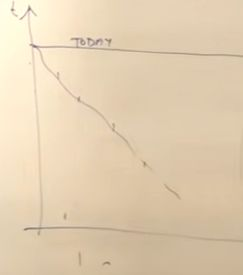
\includegraphics[width=\textwidth]{cosmo-7-universe-1}
	\end{subfigure}
	\begin{subfigure}[t]{0.45\textwidth}
		\caption{Looking back we see different time periods. The universe was optically opaque before decoupling. \gls{gls:cmb} comes from point where universe shifted from opaque. Neutrinos can come through from before. Gravitons. So, in principle, we may be able to look back further than decoupling.}
		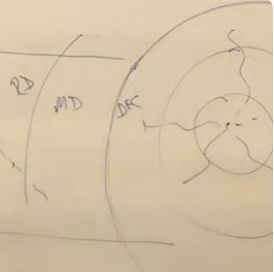
\includegraphics[width=\textwidth]{cosmo-7-universe-2}
	\end{subfigure}
\end{figure}

When temperature gets to about $10^{14}K$, $\frac{a_T}{a(t)}\approx 10^{14}$, characteristic photon energy $\epsilon_{photon}=0.5MeV$,  the $E=mc^2$ of an electron. Two photons colliding can produce electron-positron pairs; also electrons and positrons can make photons. They can form a thermal equilibrium, and are no longer determined by ''memory of the future''. Thermal equilibrium at that temperature satisfies $\gls{gls:n:electrons}=\gls{gls:n:positrons}=\gls{gls:n:gamma}$. Note that  $\gls{gls:n:electrons}-\gls{gls:n:positrons}$ does not change, but $\gls{gls:n:electrons}+\gls{gls:n:positrons}$ does: it is bigger than today's value by $10^8$.

What led to any difference?



\section{Baryogenesis}

\subsection{The Question}
Why is there so much entropy in the world? Why is the number of photons, which counts the entropy in the world\footnote{Normally the entropy is the number of photons for black body radiation}, so much higher that the number of protons and electrons($10^8\times$ larger)? Why are the protons and electrons so few? One  explanation is the Sakharov conditions: there are three of them, and, if they are satisfied, there will be an imbalance of mater over antimatter.

Is this a legitimate question? Maybe the world started with a imbalance. But numbers focus your imagination. The excess is  a fact, and maybe we could just assume it is that way.

In the very early universe there was a huge number of protons and a similar number of antiprotons (or quarks and antiquarks), ditto electrons and positrons, and ditto photons, all in thermal equilibrium. Then it cooled and the photons were left over, because they decoupled and the universe became transparent. The protons and antiprotons annihilated each other. The universe expanded slowly, so there was plenty of time for them to find each other. All that was left was the slight excess. So the question is not why there were so many photons, but why was there this slight excess of $10^{-8}$. We don't have a complete theory, but almost anything we write down always has a slight excess.

\begin{align*}
	\gls{gls:n:proton}+\gls{gls:n:electrons}-\gls{gls:n:antiproton}-\gls{gls:n:positrons} =& 0\\
	\frac{\gls{gls:n:proton}-\gls{gls:n:antiproton}}{\gls{gls:n:gamma}}\approx&10^{-8}\\
	\frac{\gls{gls:n:proton}-\gls{gls:n:antiproton}}{\gls{gls:n:proton}+\gls{gls:n:antiproton}}\approx&10^{-8}
\end{align*}

\subsection{The Old Theory}

Let us begin with a hypothesis, which is believed to be wrong. Let $B$ denote the \gls{gls:baryon:number}, \glsdesc{gls:baryon:number}. The statement that there were more protons than antiprotons is also a statement about quarks and antiquarks.
Let us suppose that \gls{gls:baryon:number} is like electric charge: it is conserved. Of course electric charge is the source of a long range force, but \gls{gls:baryon:number} is not. Protons create long range Coulomb forces, but neutrons don't. If \gls{gls:baryon:number}, then if there is an initial excess, there will always be the same excess, which will be frozen in. It appears to be highly conserved. Otherwise, what could a proton decay to?
\begin{itemize}
	\item it must decay to something lighter;
	\item it must decay to something with a positive electrical charge.
\end{itemize}
This leaves a positron and something electrically neutral, such as a photon(A neutrino is not good, as we'd have an even number of fermions). We don't know any deep fundamental reason why this can't happen.

\begin{figure}[H]
	\caption{Proton decay}
	\begin{subfigure}[b]{0.47\textwidth}
		\caption{Hypothetical scenario where a proton decays into a positron and a photon. For some reason, that Standard Model does not permit the decay , but there are extensions to the Standard Model where this could happen. We do know that the decay cannot be very fast, as the protons have been around for at least 13.7 billion years.}\label{fig:cosmo-8-proton-decay}
		\begin{center}
			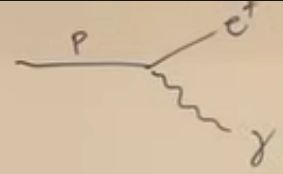
\includegraphics[width=\textwidth]{cosmo-8-proton-decay}
		\end{center}
	\end{subfigure}
	\begin{subfigure}[b]{0.47\textwidth}
		\caption{Somewhere in the guts of the Feynman diagram, assume there is a very, very heavy particle, outside the Standard Model, say $10^{16}GeV$, then the process is very slow, and is suppressed by powers of the heavy mass.}\label{fig:cosmo-8-proton-decay-mechanism}
		\begin{center}
			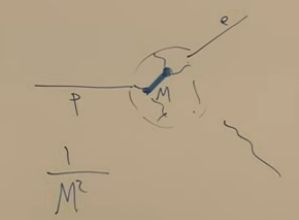
\includegraphics[width=\textwidth]{cosmo-8-proton-decay-mechanism}
		\end{center}
	\end{subfigure}	
\end{figure}

For some reason, that Standard Model does not permit the decay in Figure \ref{fig:cosmo-8-proton-decay}, but there are extensions to the Standard Model where this could happen. We do know that the decay cannot be very fast, as the protons have been around for at least 13.7 billion years. So we think that the excess has been built in from the very beginning.

There is another symmetry of nature that isn't really a symmetry. Sakharov wrote a couple of years after it was discovered that it wasn't a symmetry: particle-antiparticle reflection symmetry. This says that if particles are replaced with reflection we can't tell the difference.

Until the 1960s it was believed that the following 3 symmetries existed:
\begin{itemize}
	\item Charge Conjugation, $C$;
	\item Parity $P$;
	\item Time $T$.
\end{itemize} 

We now know that the symmetry is $CPT$ (In the Scr\"odinger equation, $t\rightarrow-t, \psi\rightarrow\psi^{*}, i\rightarrow -i$).

\begin{align*}
	i \hbar \frac{\partial \psi}{\partial t} =& \big[-\frac{\hbar}{2m} \frac{\partial^2 }{\partial x^2} + V(x)\big]\psi\\
	-i \hbar \frac{\partial \psi^*}{\partial (-t)} =& \big[-\frac{\hbar}{2m} \frac{\partial^2 }{\partial (-x)^2} + V(-x)\big]\psi^*
\end{align*}
Imagine (before Sakharov) that $CP$ was a symmetry: then you might be able to swap particles and antiparticles and reflect left \& right. But if there were a complete symmetry, why the imbalance? It doesn't sound right.

\subsection{The Sakharov Conditions}

\begin{enumerate}
	\item \gls{gls:baryon:number} violation
	\item C-symmetry and CP-symmetry violation.
	\item Interactions out of thermal equilibrium, breaking T symmetry.
\end{enumerate}

\subsubsection{\gls{gls:baryon:number} violation}
 This begins with the idea that there \emph{was} a balance: that there was no bias towards particles or antiparticles. The only way to get unbalanced is if conservation of \gls{gls:baryon:number} is not correct. If something like Figure \ref{fig:cosmo-8-proton-decay} can happen, the number of protons can change. The first requirement for a theory that starts with balance is to have a mechanism that violates conservation. That was the first of the Sakharov conditions.

 If \gls{gls:baryon:number} conservation is not a good symmetry, it must be very weakly broken, and have a very small probability per unit time, since protons are very, very old. Every known unified theory violates \gls{gls:baryon:number} conservation.  You might ask why, in the known theories, the proton is so stable. Somewhere in the guts of the Feynman diagram, Figure \ref{fig:cosmo-8-proton-decay-mechanism}, assume there is a very, very heavy particle, outside the Standard Model, say $10^{16}GeV$, then the process is very unlikely, and its amplitude is suppressed by powers of the heavy mass.
 
 If the proton has extra energy, the factor of $\frac{1}{M^2}$ in Figure \ref{fig:cosmo-8-proton-decay-mechanism} becomes $\frac{1}{(M-E)^2}$, so there will be less suppression ($Energy=m c^2 + E$). Normally $E$ is negligible. Theories of this type can explain stability.
 
 All current theories include the \emph{possibility} of Baryon violation.
  Very hot at beginning! But Baryon violation by itself isn't enough by itself to give an average excess of protons over antiprotons: for every event like  Figure \ref{fig:cosmo-8-proton-decay}, which reduces baryon number, there is a charge conjugated process that increases baryon number--Figure \ref{fig:cosmo-8-anti-proton-decay}. 
 
 \begin{figure}[H]
 	\caption{cosmo-8-anti-proton-decay}\label{fig:cosmo-8-anti-proton-decay}
 	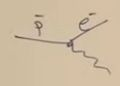
\includegraphics[width=0.5\textwidth]{cosmo-8-anti-proton-decay}
 \end{figure}
 
 If we believe in particle-antiparticle symmetry, on average there will be as many Figure \ref{fig:cosmo-8-anti-proton-decay} decays as Figure \ref{fig:cosmo-8-proton-decay}. the process could decay antiprotons, or run in reverse. If we started with an equal population of quarks and antiquarks, and try to rely only on violation of Baryon number, it would not be an efficient way to create an excess. Moreover, in the very early universe there were lots of electrons, positrons and photons, so it was possible for the reactions to go backwards. There is a statistical process going on, so it is only statistical that there would be as many protons as antiprotons. The excess of protons over antiprotons cannot be a statistical effect.
 
 It is quite true that the excess is a small number, $10^{-8}$, but how many protons are there in the observable universe? About $10^{80}$. How big would you expect it to be if it were a pure statistical effect? $\sqrt{N}$ is the expected fluctuation in a variable. In a world with $10^{80}$ protons, we'd expect a fluctuation of $\sqrt{10^{80}}=\sqrt{10^{40}}$. If excess were around this size it might be statistical.
 
 If it were statistical fluctuation, it would be hard to understand why it is the same everywhere. If there were anti-galaxies, we'd expect high energy cosmic rays to have as many anti-nuclei as nuclei\footnote{LS believes that Helium niclei have been seen in cosmic rays.}. We don't see this. (We do see antiprotons, however, but they can be explained by collisions in the upper atmosphere).
 
 If our galaxy were particles, and the Andromeda galaxy were antimatter, we'd expect to see a lot of annihilation in between.
 
 
\subsubsection{C and CP violation} 

Particle-antiparticle symmetry \emph{suggests} that the universe was created symmetrically, although it doesn't prove it. In order to account for the lack of symmetry between particles and antiparticles, this charge conjugation symmetry must fail, as must CP symmetry.	 Baryon violation isn't enough: we need something to push it in a particular direction. We need bias. We need violations of Particle-Antiparticle symmetry, and both C and CP  symmetry.

Is there evidence of violation of particle-antiparticle symmetry? We have experimental evidence that particles and antiparticles don't behave the same way. The simplest example is the B meson, which is made of a bottom quark and an anti-down quark: it has an anti-particle. \begin{itemize}
	\item $B\rightarrow K^+ + \pi^-$ 
	\item $\bar{B}\rightarrow K^- + \pi^+$ 
\end{itemize}
 
 The rates for these to happen are measurable, and they are different.
 
 
 \subsubsection{T symmetry broken}
 We have CPT symmetry in all known theories. In thermal equilibrium backward and forward time are the same; so we have T symmetry, so CPT symmetry gives CP symmetry. But expanding universe not in equilibrium. In a rapidly expanding universe, T symmetry is broken. Must be fast! But then suddenly slowed.


 These appear to be true, and they are sufficient to explain excess. But nobody knows enough to make a calculation of imbalance--$10^-8$
 \url{https://youtu.be/gdFldkitkJA?t=1664}
 \url{https://youtu.be/gdFldkitkJA?t=3867}
 
\section{Inflation}

\begin{quotation}
	Professor Susskind introduces the theory of cosmological inflation under which the early universe underwent an exponential expansion during which it doubled in size every 10-32 seconds and expanded by at least a factor of $e^{90}$.  This all occurred prior to the Big Bang and during this period the universe cooled very rapidly and was essentially empty.  In the early phase of this rapid expansion, the universe was hot enough that magnetic monopoles were formed.  However these were the only particles formed.  The rest of the energy of the universe was contained in the potential energy of the inflaton field, and it wasn't until the Big Bang that this potential energy was converted into the particles that form the matter that makes up the galaxies in the universe today.
	
	This theory of rapid expansion explains the lack of observed magnetic monopoles and the uniformity of the \gls{gls:cmb} radiation.  The rapid expansion dispersed the monopoles, smoothed out the distribution of photons, and also flattened space itself.
	
\end{quotation}

\section{Inhomogeneities and quantum fluctuations}

\begin{quotation}
Professor Susskind describes the theory whereby inhomogeneities in the universe were caused by quantum fluctuations in the early universe.  He begins with the mathematical equations of a damped harmonic oscillator, and relates that simple system to a dissipative inflation field with spatial dependencies.  The quantum fluctuations in the zero point energy states of this field lead to inhomogeneities in the universe.  These inhomogeneities explain both the small variations in the \gls{gls:cmb}, as well as the formation of galaxies from regions of high energy density.
\end{quotation}


% glossary: may need command makeglossaries.exe cosmology
\printglossaries

\bibliographystyle{unsrt}
\addcontentsline{toc}{section}{Bibliography}
\raggedright
\bibliography{tm}

\end{document}
